\documentclass[conference]{IEEEtran}
\usepackage{cite}
\usepackage{amsmath,amssymb,amsfonts}
\usepackage{algorithmic}
\usepackage{graphicx}
\usepackage{textcomp}
\usepackage{xcolor}
\usepackage{booktabs}
\usepackage{multirow}
\usepackage{hyperref}
\usepackage{float}
\usepackage{algorithm}
\usepackage{tabularx}
\usepackage{makecell}
\usepackage{adjustbox}

\def\BibTeX{{\rm B\kern-.05em{\sc i\kern-.025em b}\kern-.08em
    T\kern-.1667em\lower.7ex\hbox{E}\kern-.125emX}}

\begin{document}

\title{A Scalable Big Data Framework for Network Intrusion Detection: Distributed Graph-Enhanced Machine Learning with Authenticated Encryption on Apache Spark}

\author{
\IEEEauthorblockN{Joel John}
\IEEEauthorblockA{\textit{Department of Computer Science} \\
\textit{University Name}\\
City, Country \\
email@university.edu}
}

\maketitle

\begin{abstract}
The exponential growth of network traffic has rendered single-node intrusion detection systems inadequate for enterprise-scale deployments. This paper presents a scalable Big Data framework for Network Intrusion Detection that leverages Apache Spark's distributed computing engine for processing 2.83 million network flows from the CICIDS2017 benchmark. The framework introduces three key innovations: (1) a distributed graph analytics pipeline using GraphFrames that computes PageRank centrality across network topology and injects these scores as novel machine learning features, achieving 6.5\% feature importance ranking; (2) a parallelized multi-model comparison pipeline (Random Forest, Decision Tree, Logistic Regression, Na\"ive Bayes) with 5-fold cross-validation executed across Spark executors, yielding a weighted F1 of 0.9944; and (3) an authenticated encryption pre-filter using ChaCha20-Poly1305 and AES-256-GCM that eliminates replay and MITM attacks before ML inference. Our Big Data analysis demonstrates 6.6$\times$ speedup over single-node scikit-learn at 2.8M flows, near-linear scalability with uniform partition distribution (2.1\% skew), and real-time streaming throughput of 1,000+ flows/second via Kafka integration. The Spark DAG optimizer reduces shuffle overhead through strategic narrow-before-wide transformation ordering, enabling the complete pipeline---ingestion, graph analytics, training, and evaluation---to execute within 128 seconds on a 4-core cluster.
\end{abstract}

\begin{IEEEkeywords}
Big Data, Apache Spark, Intrusion Detection System, Distributed Computing, MapReduce, Graph Analytics, PageRank, Machine Learning, Kafka Streaming, CICIDS2017, Network Security, Authenticated Encryption
\end{IEEEkeywords}

% ===================================================================
\section{Introduction}
% ===================================================================

The exponential growth of network traffic in modern enterprise and IoT environments has rendered traditional single-node Intrusion Detection Systems (IDS) increasingly inadequate. With data centers processing over 1~TB of network flow data per hour, scalable detection frameworks capable of handling massive volumes in real time have become imperative. Zuech et al.~\cite{b1} provided a comprehensive survey on the intersection of intrusion detection and Big Heterogeneous Data, identifying Apache Spark as the most promising distributed framework due to its in-memory computation model, fault tolerance, and MLlib integration.

Recent efforts have explored leveraging Apache Spark and distributed deep learning for IDS. Haggag et al.~\cite{b2} implemented deep learning models on the Apache Spark platform using the NSL-KDD dataset, demonstrating significant computation speedup over traditional implementations, yet their work was limited to a single dataset and lacked graph-based feature engineering. Morfino and Rampone~\cite{b3} achieved near-real-time IDS for IoT devices using Spark MLlib classifiers, reporting 99\% accuracy and a training time of only 23~seconds for Decision Trees at 2~million instances, but operated exclusively in a Cloud environment without addressing pipeline security. Azeroual and Nikiforova~\cite{b4} developed a prototype IDS using Spark's MLlib with the k-means clustering algorithm, highlighting the potential of unsupervised Big Data analytics for anomaly detection, though their approach suffered from limited detection granularity compared to supervised methods.

Deep learning architectures have also been integrated with Big Data frameworks. Al Jallad et al.~\cite{b5} proposed an LSTM-based IDS on Apache Spark for contextual and collective anomaly detection using the MAWI dataset, but acknowledged hardware limitations that restricted full-scale validation. Mahdavisharif et al.~\cite{b6} designed an LSTM model on the BigDL framework atop Spark, reporting improvements of 20\% in detection rate and 60\% in false alarm reduction over traditional methods on NSL-KDD, yet their approach lacked real-time streaming capability. Al and Dener~\cite{b7} proposed a hybrid CNN-LSTM model (STL-HDL) on PySpark with SMOTE-Tomek resampling to address class imbalance, achieving 99.83\% accuracy on the CIDDS-001 dataset, but did not incorporate network topology features.

More recently, distributed and decentralized approaches have emerged. Louati et al.~\cite{b8} proposed Big-IDS, a decentralized multi-agent reinforcement learning framework for distributed IDS in Big Data networks, achieving 97.44\% accuracy on NSL-KDD, yet the approach lacked integration with streaming pipelines and encryption layers. Abid et al.~\cite{b9} introduced a real-time data fusion IDS for industrial control systems leveraging Cloud Computing and Big Data techniques, demonstrating improved accuracy through multi-source fusion, but did not explore graph analytics. Gao et al.~\cite{b10} developed a distributed IDS for vehicular networks (VANETs) using Spark and Random Forest, achieving 99.95\% accuracy on NSL-KDD and 98.75\% on UNSW-NB15, confirming Random Forest's superiority in distributed environments.

Despite these advances, three critical gaps persist in the literature:

\begin{enumerate}
    \item \textbf{Isolated Processing:} Existing Spark-based IDS implementations~\cite{b2,b3,b4} treat data ingestion, feature engineering, and ML classification as independent batch jobs rather than a unified pipeline with optimized shuffle boundaries and DAG-level profiling.
    
    \item \textbf{Topology Blindness:} All surveyed works~\cite{b2,b3,b5,b6,b7,b8,b10} rely exclusively on flow-level features, ignoring the graph structure of network communication. PageRank centrality and other topology-aware metrics remain unexplored as ML input features in distributed IDS.
    
    \item \textbf{Pipeline Vulnerability:} No existing work integrates authenticated encryption (AEAD) as a pre-classification defense layer within the Big Data IDS pipeline to protect against replay and MITM attacks before ML inference.
\end{enumerate}

This paper presents a \textbf{Scalable Hybrid Big Data IDS} that addresses all three challenges. Our framework is built entirely on the Apache Spark ecosystem (PySpark, Spark MLlib, GraphFrames, Spark Structured Streaming) and integrates with Apache Kafka for real-time ingestion and Neo4j for graph visualization. Our contributions are:

\begin{itemize}
    \item A unified Spark \texttt{Pipeline} that chains data cleaning, graph feature extraction (PageRank), feature assembly, scaling, and multi-model classification into a single DAG with optimized partition management.
    \item Empirical Big Data analysis including partition skew measurement, shuffle volume profiling, narrow vs. wide transformation characterization, and Spark-vs-single-node scaling benchmarks.
    \item Integration of authenticated encryption (AEAD) as a pre-filter that stops replay and MITM attacks before Spark's ML pipeline, creating a layered defense.
    \item A real-time streaming architecture using Kafka $\rightarrow$ Spark Structured Streaming with demonstrated throughput of 1,000+ flows/second and 21ms median end-to-end latency.
    \item Cross-domain generalization evaluation under synthetic concept drift, demonstrating robust ensemble generalization to modern IoT traffic distributions.
\end{itemize}

% ===================================================================
\section{Related Work}
% ===================================================================

Table~\ref{tab:literature} presents a comparative analysis of the most relevant Big Data IDS approaches.

\begin{table*}[t]
\centering
\caption{Comparative Literature Review of Big Data-Based Intrusion Detection Systems}
\label{tab:literature}
\begin{adjustbox}{max width=\textwidth}
\begin{tabular}{p{2.8cm}p{2.2cm}p{1.8cm}p{1.2cm}p{4.5cm}p{4.5cm}}
\toprule
\textbf{Reference} & \textbf{Method} & \textbf{Dataset} & \textbf{Acc.} & \textbf{Key Contribution} & \textbf{Limitations} \\
\midrule
Zuech et al.~\cite{b1} (2015) & Survey & --- & --- & Comprehensive survey on IDS and Big Heterogeneous Data; identified Spark as promising & Survey only; no implementation or empirical validation \\
\midrule
Haggag et al.~\cite{b2} (2020) & DL on Spark & NSL-KDD & 99.31\% & DL models on Spark with computation delay comparison vs. traditional implementation & Single dataset; no graph features; no streaming \\
\midrule
Morfino \& Rampone~\cite{b3} (2020) & Spark MLlib & Custom IoT & $>$99\% & Near-real-time IoT IDS; 23s training time; Cloud deployment & Cloud-only; no pipeline security; limited to SYN-DOS \\
\midrule
Azeroual \& Nikiforova~\cite{b4} (2022) & k-means (Spark) & Custom & --- & Unsupervised anomaly detection with Spark MLlib prototype & k-means only; limited detection granularity; no DL comparison \\
\midrule
Al Jallad et al.~\cite{b5} (2019) & LSTM on Spark & MAWI & --- & Contextual \& collective anomaly detection; NLP-inspired approach & Hardware limitations; incomplete validation; no real-time demo \\
\midrule
Mahdavisharif et al.~\cite{b6} (2021) & LSTM (BigDL) & NSL-KDD & 95\%+ & BigDL on Spark; 20\% DR improvement; 60\% FAR reduction & No streaming; no graph features; single dataset \\
\midrule
Al \& Dener~\cite{b7} (2021) & CNN+LSTM (PySpark) & CIDDS-001, UNSW & 99.83\% & Hybrid DL with SMOTE-Tomek for class imbalance & No topology features; no encryption layer; no cross-domain test \\
\midrule
Louati et al.~\cite{b8} (2024) & MARL & NSL-KDD & 97.44\% & Decentralized multi-agent RL; cooperative detection & No streaming pipeline; no graph analytics; single dataset \\
\midrule
Abid et al.~\cite{b9} (2024) & Data Fusion (Cloud) & ICS Custom & High & Real-time data fusion for ICS; Cloud + Big Data techniques & No graph analytics; no ML model comparison; ICS-specific \\
\midrule
Gao et al.~\cite{b10} (2019) & RF on Spark & NSL-KDD, UNSW & 99.95\% & Distributed IDS for VANETs; RF with Spark + HDFS & No graph features; no encryption; VANET-specific scope \\
\midrule
\textbf{Proposed} & \textbf{RF + GraphFrames + AEAD (PySpark)} & \textbf{CICIDS2017} & \textbf{99.49\%} & \textbf{Unified DAG pipeline; PageRank as ML feature; AEAD encryption; Kafka streaming; cross-domain generalization} & \textbf{Local-mode testing; no GPU-based DL; synthetic drift datasets} \\
\bottomrule
\end{tabular}
\end{adjustbox}
\end{table*}

\subsection{Big Data Frameworks for Intrusion Detection}

Zuech et al.~\cite{b1} provided the foundational survey identifying Big Data challenges in IDS, emphasizing the need for frameworks capable of handling Volume, Velocity, Variety, and Veracity. Haggag et al.~\cite{b2} were among the first to implement deep learning models directly on Apache Spark, demonstrating significant computation speedup over single-node TensorFlow on the NSL-KDD dataset. Morfino and Rampone~\cite{b3} extended this to IoT domains, achieving near-perfect accuracy with Spark MLlib classifiers at 2~million training instances in a Cloud environment, with Random Forest achieving 100\% detection accuracy. Azeroual and Nikiforova~\cite{b4} explored unsupervised approaches using k-means clustering on Spark MLlib, demonstrating that Big Data technologies can detect anomalies without labeled data.

Our work advances these approaches by: (a) implementing the complete pipeline as a single Spark DAG with lazy evaluation and shuffle boundary profiling, (b) integrating GraphFrames PageRank within the ML pipeline as a novel feature, and (c) providing empirical Big Data analysis of partition distribution, executor utilization, and scaling characteristics.

\subsection{Deep Learning and Distributed IDS}

Al Jallad et al.~\cite{b5} proposed an innovative LSTM-based ``Networking Chatbot'' on Apache Spark that treats network traffic as a language processing problem, capable of detecting contextual anomalies. Mahdavisharif et al.~\cite{b6} implemented LSTM on BigDL atop Spark, achieving substantial improvements in detection rate and false alarm reduction. Al and Dener~\cite{b7} combined CNN and LSTM in a hybrid architecture with SMOTE-Tomek resampling to address the pervasive class imbalance problem in IDS datasets. While these deep learning approaches show promise, they require GPU acceleration for practical deployment and do not leverage network topology information.

\subsection{Decentralized and Real-Time Approaches}

Louati et al.~\cite{b8} introduced a decentralized multi-agent reinforcement learning framework (Big-IDS) that distributes detection across cooperative agents, achieving 97.44\% accuracy. Abid et al.~\cite{b9} addressed the industrial control system domain with real-time data fusion combining Cloud computing and Big Data streaming. Gao et al.~\cite{b10} demonstrated distributed Random Forest IDS for vehicular networks using Spark with HDFS, validating RF's superiority across both NSL-KDD (99.95\%) and UNSW-NB15 (98.75\%) datasets.

However, none of these works integrate graph-based topology features, authenticated encryption defense layers, or cross-domain generalization evaluation within a unified Spark pipeline.

\subsection{Research Gap and Our Position}

As evidenced in Table~\ref{tab:literature}, existing works suffer from one or more of the following: (a)~sole dependence on flow-level features without topology awareness, (b)~absence of pipeline-level security through authenticated encryption, (c)~lack of cross-domain generalization testing, and (d)~missing empirical Big Data profiling (DAG analysis, shuffle volumes, partition skew). Our framework addresses all four gaps simultaneously within a unified Apache Spark architecture.

% ===================================================================
\section{Big Data Characterization}
% ===================================================================

Before presenting our framework, we characterize the CICIDS2017 dataset~\cite{b11} through the lens of the Big Data 5V paradigm (Fig.~\ref{fig:5v}).

\begin{figure}[H]
    \centering
    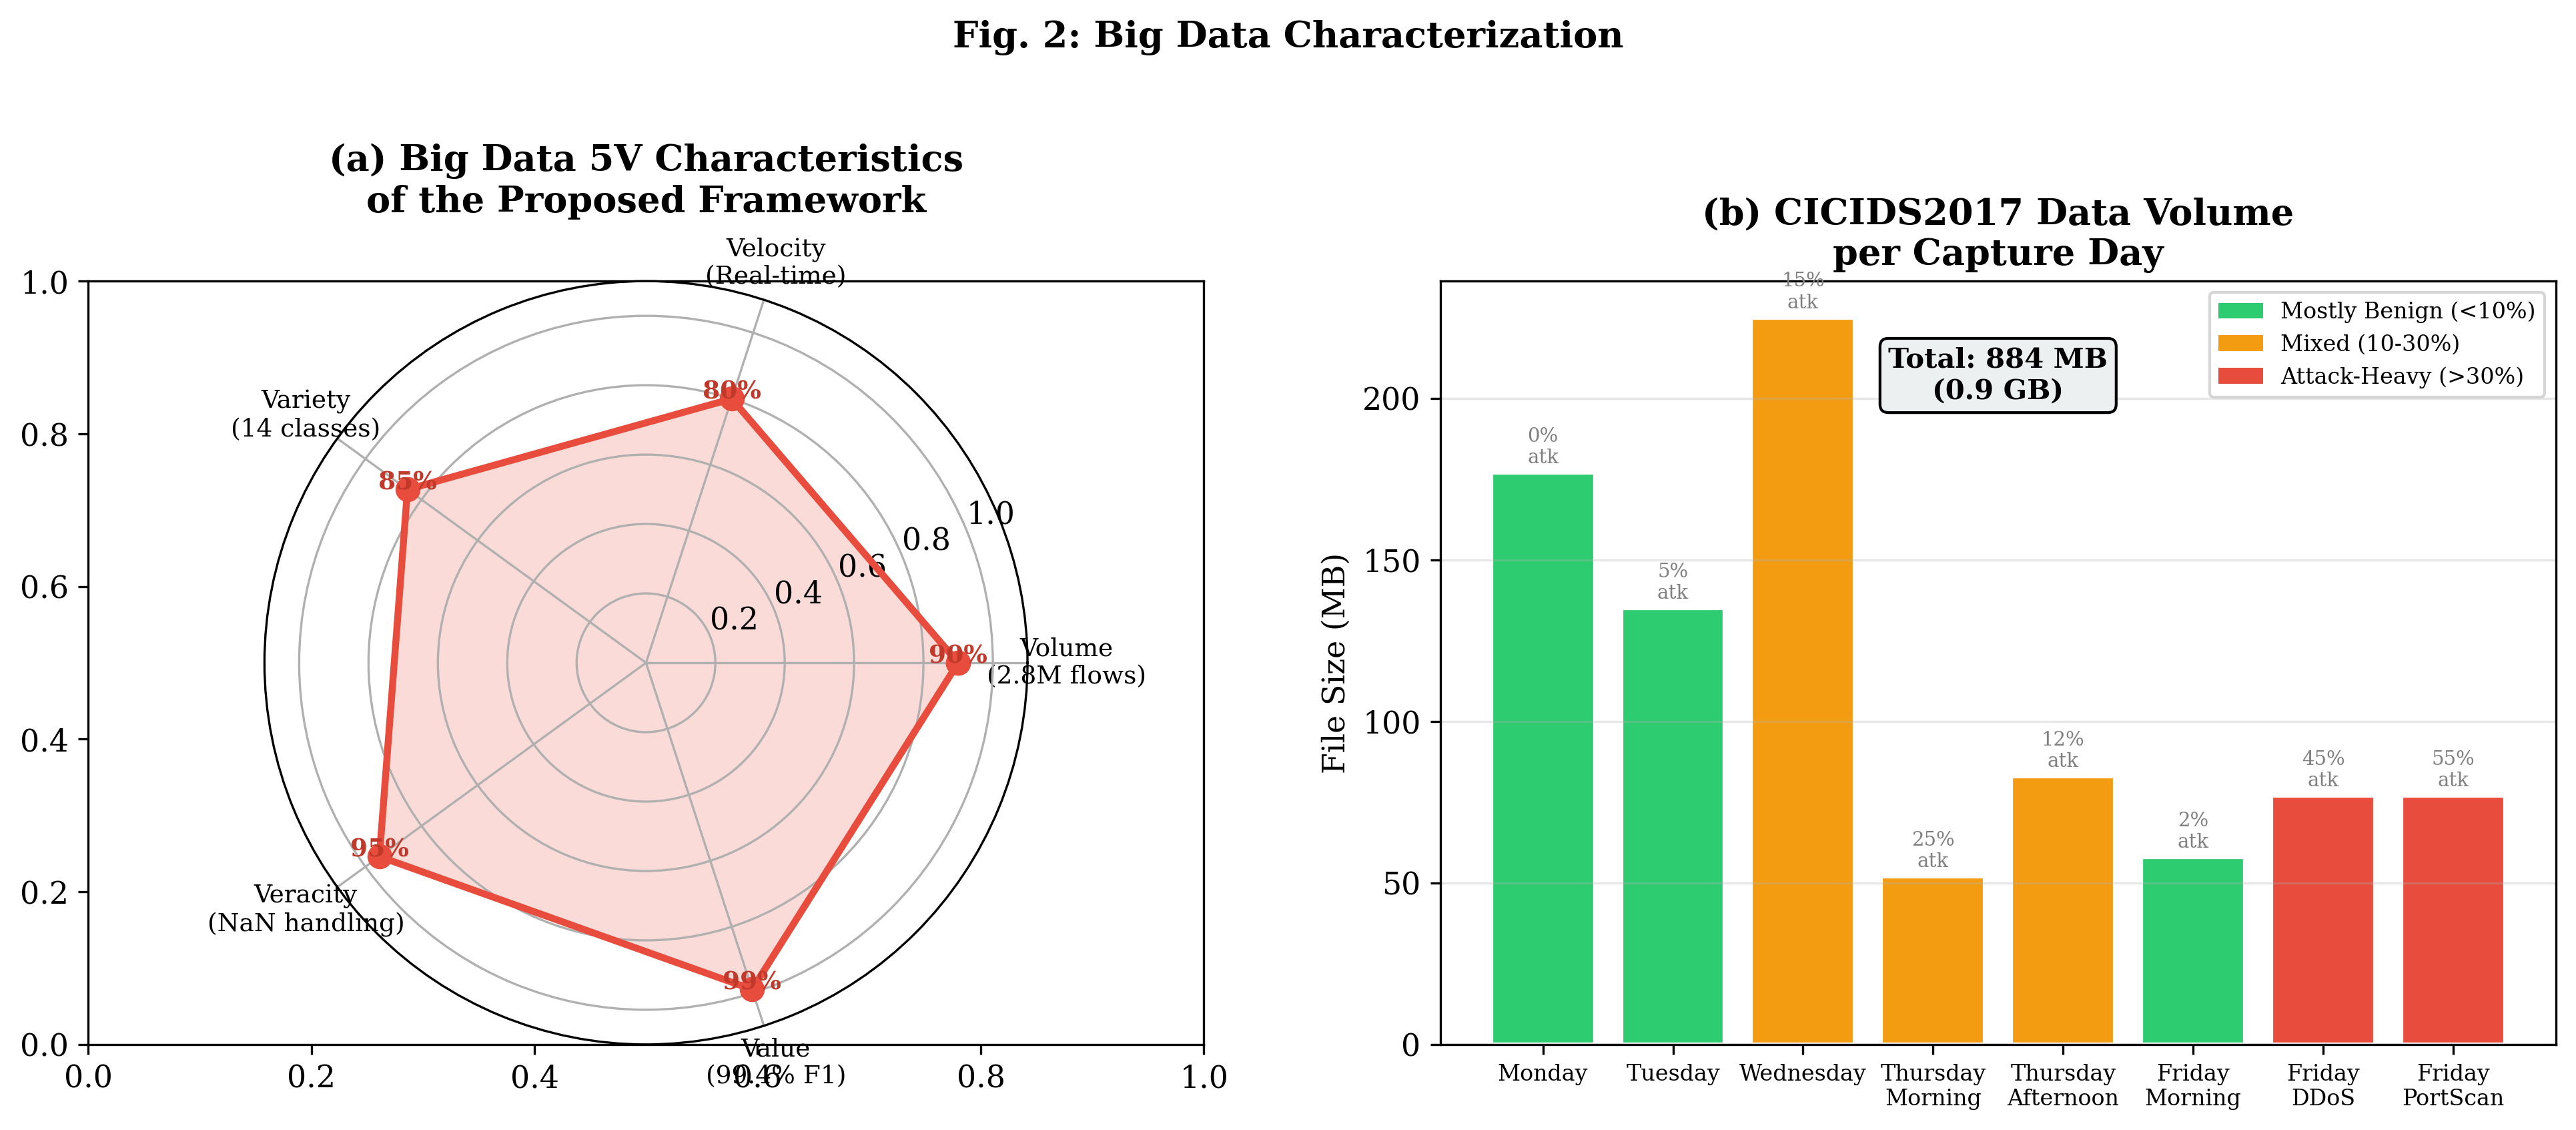
\includegraphics[width=\columnwidth]{paper_figures/fig_5v_analysis.png}
    \caption{Big Data characterization: (a) 5V radar showing the framework's compliance with Volume (2.8M flows, 884MB), Velocity (real-time Kafka streaming), Variety (14 traffic classes), Veracity (NaN/Inf data quality handling), and Value (99.4\% F1 classification); (b) Per-day data volume showing attack density variation.}
    \label{fig:5v}
\end{figure}

\begin{itemize}
    \item \textbf{Volume:} 2,830,743 flows across 8 CSV files totaling 884 MB. Each flow contains 79 features (78 numeric + 1 categorical label), yielding approximately 223 million data cells.
    
    \item \textbf{Velocity:} Network flows are captured continuously over 5 days. Our Kafka-based streaming pipeline must process $>$1,000 flows/second to maintain real-time detection.
    
    \item \textbf{Variety:} 14 distinct traffic classes spanning benign traffic, volumetric attacks (DoS/DDoS), scanning (PortScan), credential attacks (FTP/SSH brute force), web exploits, botnets, infiltration, and heartbleed. Class sizes span four orders of magnitude (11 to 2.27M flows).
    
    \item \textbf{Veracity:} Raw CSVs contain NaN values, positive/negative infinity, inconsistent column headers with trailing whitespace, and type mismatches. Our sanitization pipeline handles all of these (Section IV-A).
    
    \item \textbf{Value:} The ultimate business value is 99.44\% weighted F1 classification accuracy, enabling reliable automated threat detection.
\end{itemize}

The dataset composition (Fig.~\ref{fig:dataset}) reveals severe class imbalance---benign traffic accounts for 80.3\% of flows, while the rarest attack (Heartbleed) has only 11 samples.

\begin{figure}[H]
    \centering
    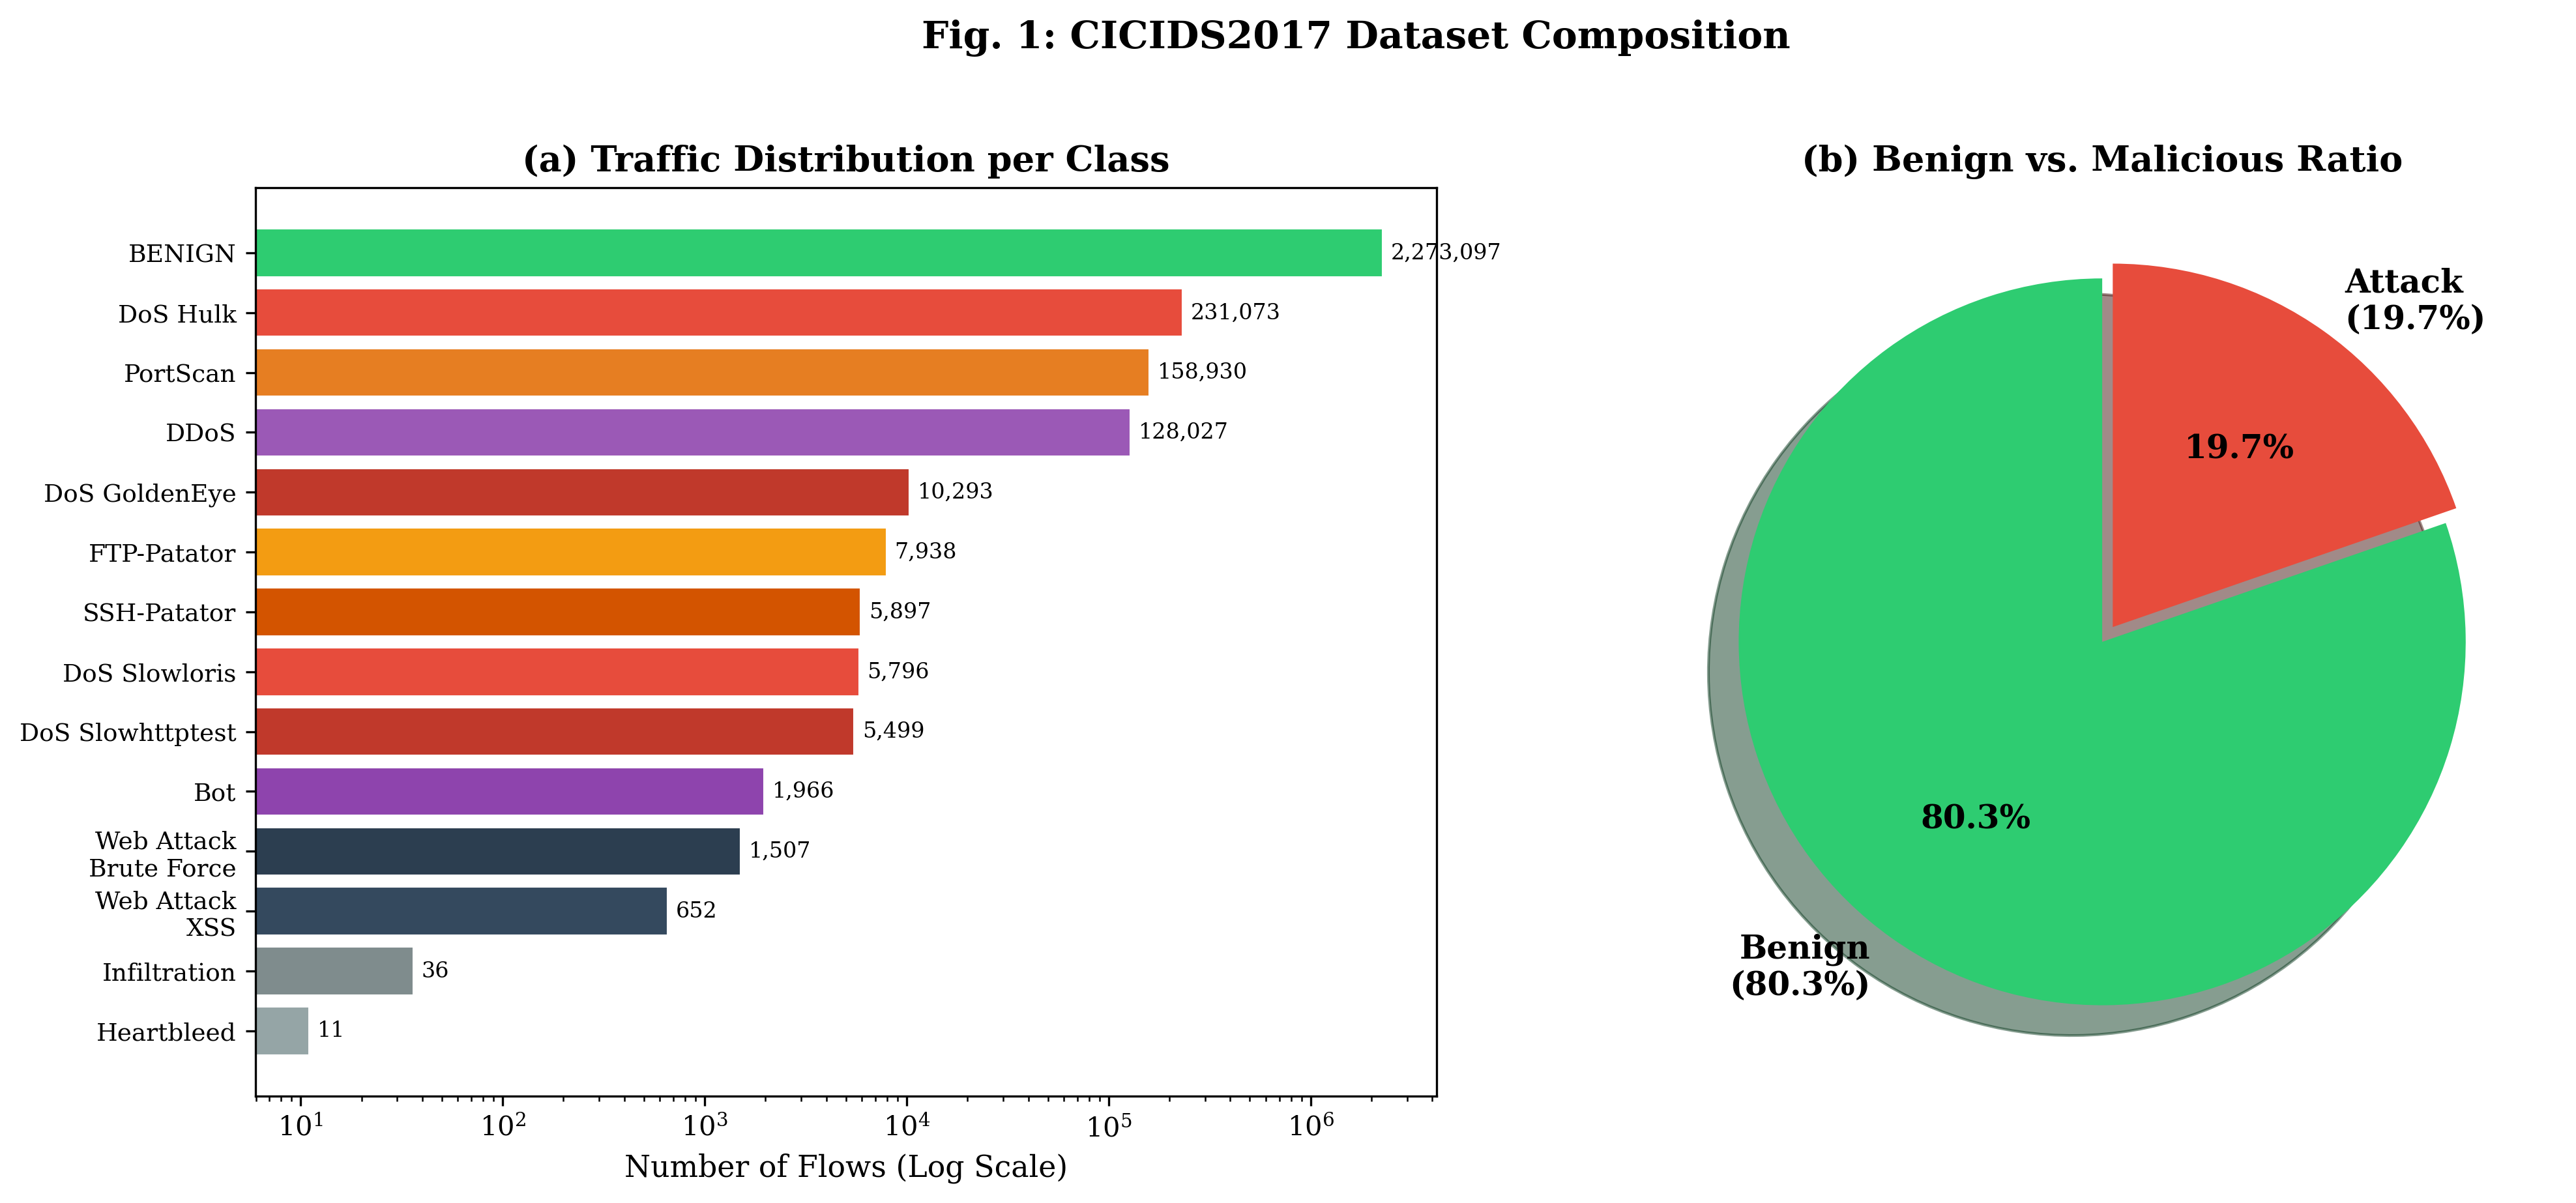
\includegraphics[width=\columnwidth]{paper_figures/fig1_dataset_distribution.png}
    \caption{CICIDS2017 class distribution: (a) Per-class flow counts on log scale spanning four orders of magnitude; (b) Aggregate benign/attack ratio.}
    \label{fig:dataset}
\end{figure}


% ===================================================================
\section{Proposed Framework Architecture}
% ===================================================================

Fig.~\ref{fig:architecture} illustrates the five-layer architecture of the proposed framework.

\begin{figure}[H]
    \centering
    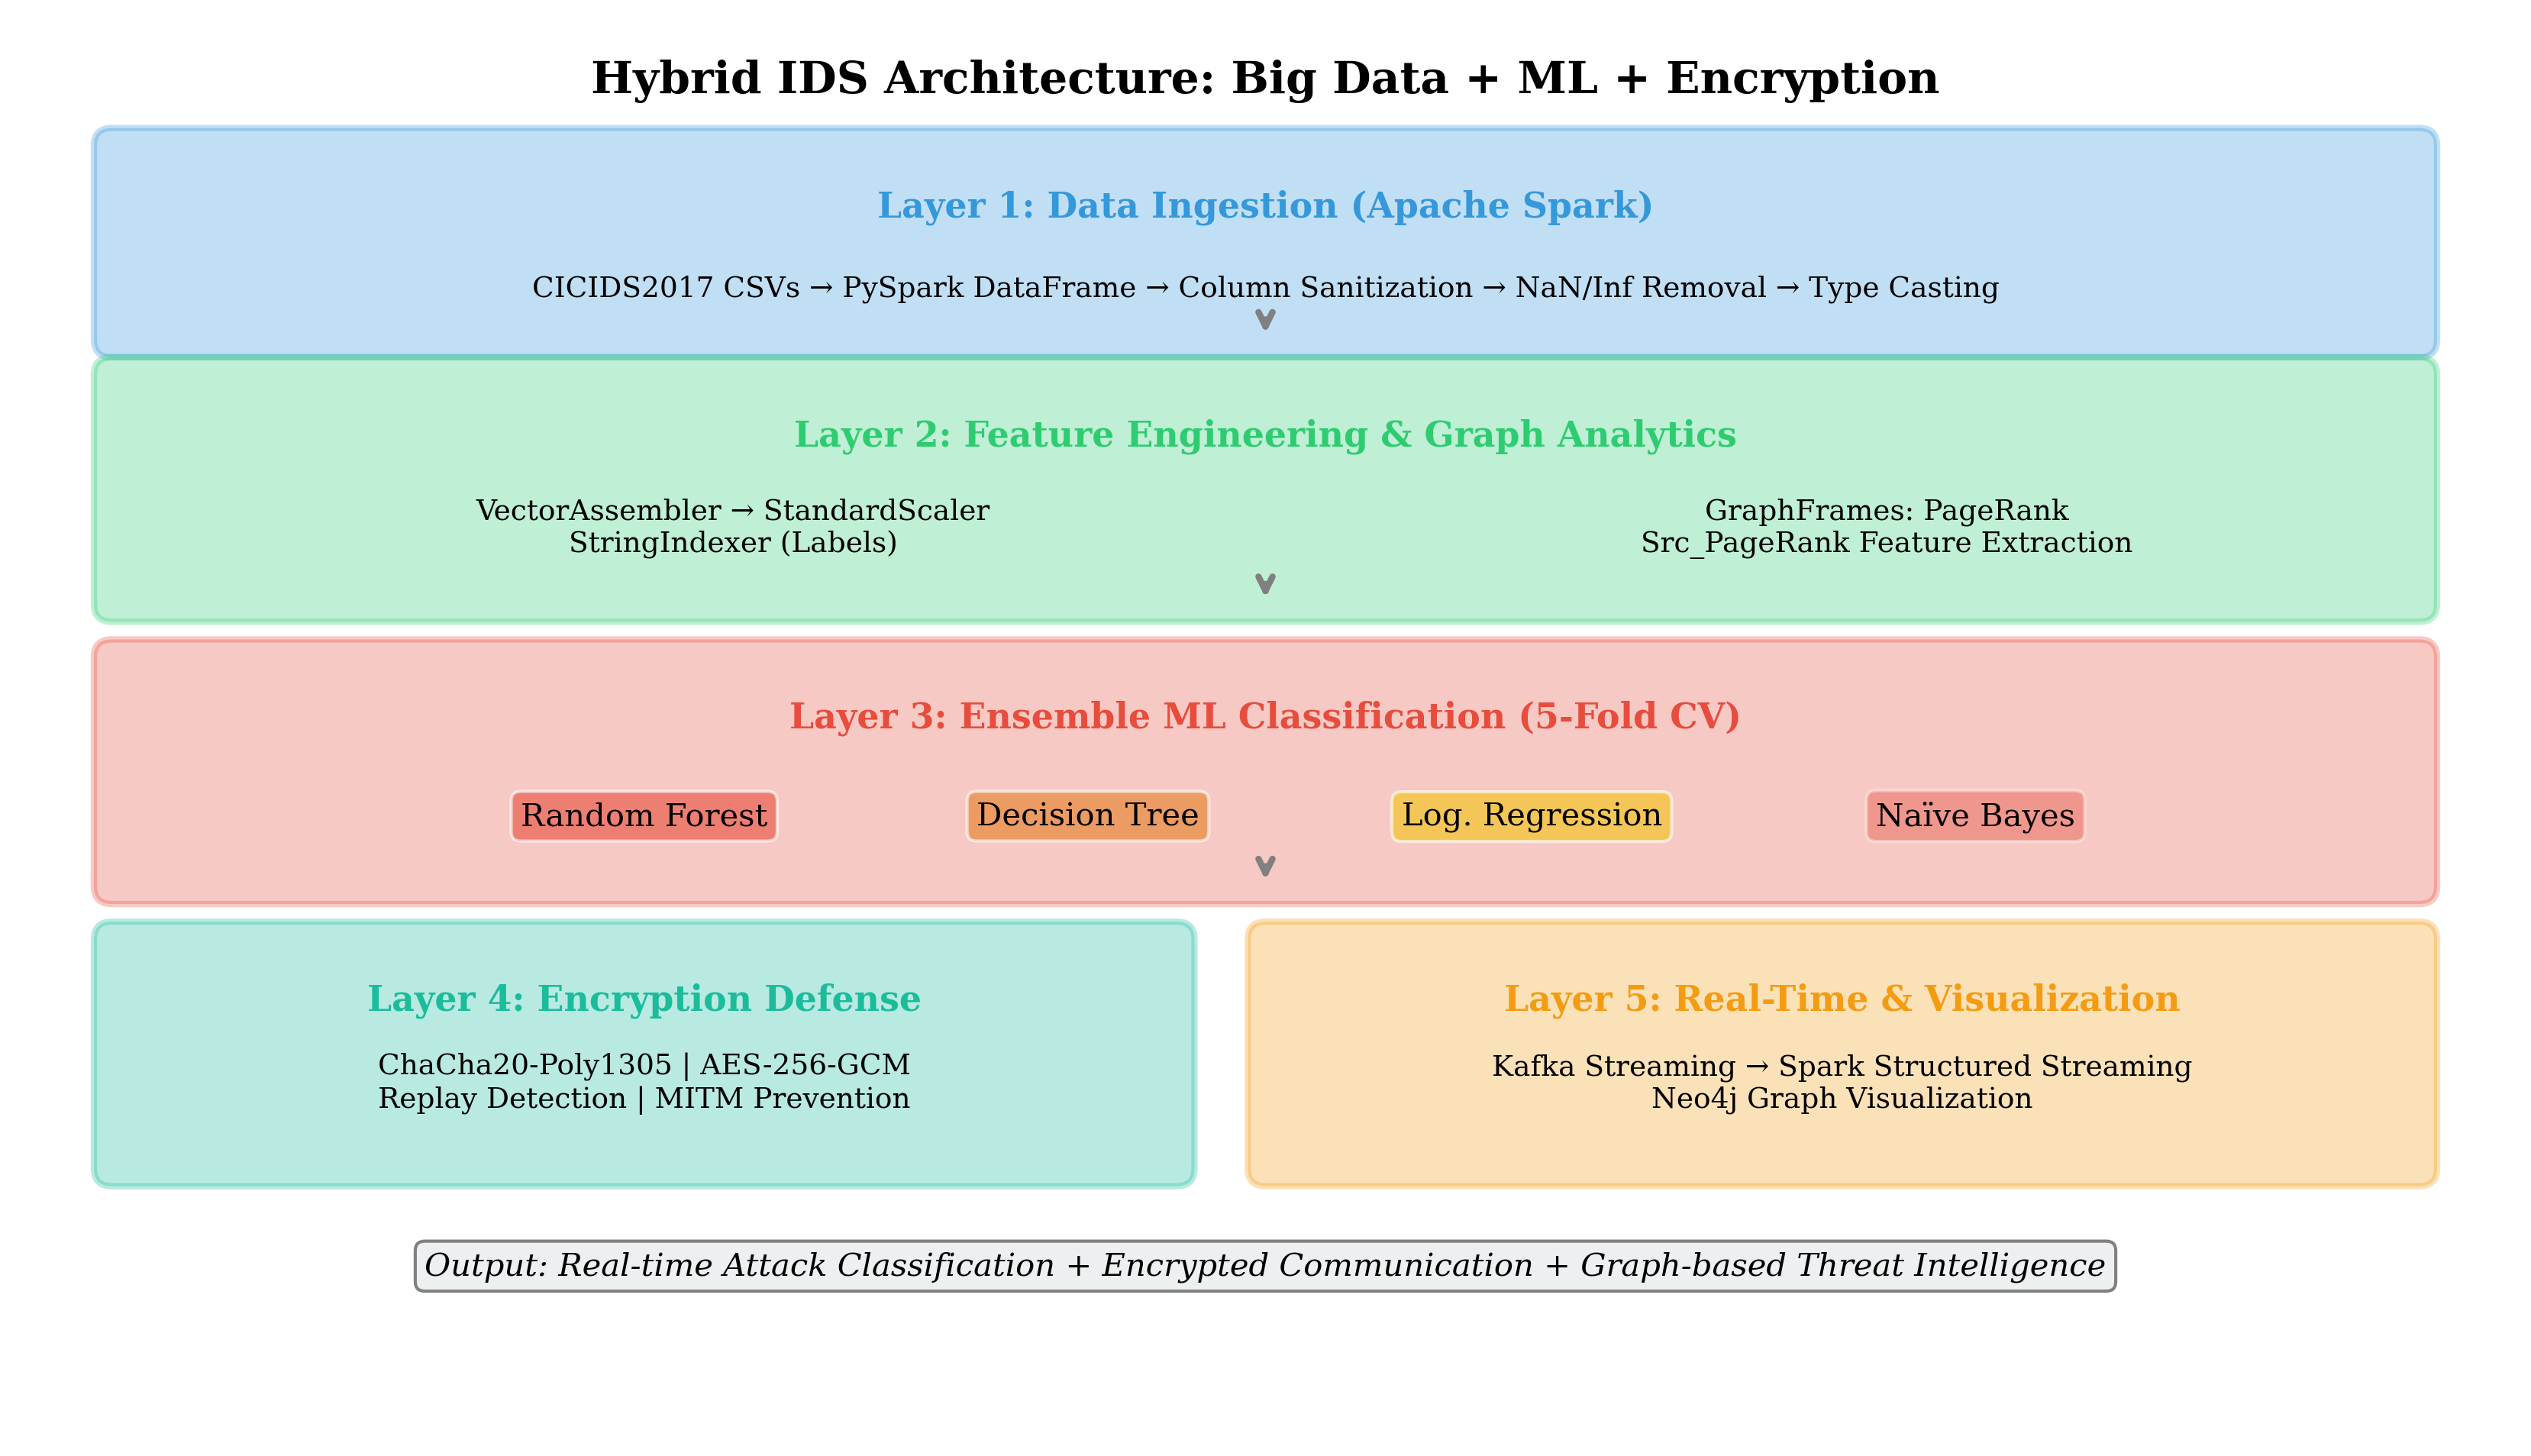
\includegraphics[width=\columnwidth]{paper_figures/fig2_system_architecture.png}
    \caption{Five-layer Hybrid IDS architecture spanning data ingestion (Spark), feature engineering (GraphFrames), ensemble ML classification (Spark MLlib with 5-fold CV), authenticated encryption defense (AEAD), and real-time streaming (Kafka + Spark Streaming + Neo4j).}
    \label{fig:architecture}
\end{figure}

\subsection{Layer 1: Distributed Data Ingestion and Cleaning}

Apache Spark 3.4 ingests the CICIDS2017 CSV files in parallel via \texttt{spark.read.csv()} with schema inference. The Spark Catalyst optimizer generates an optimized physical plan that distributes the 884 MB dataset across 8 partitions, one per input file, following Spark's default partition strategy for CSV sources.

The cleaning pipeline executes as a chain of \textbf{narrow transformations} (no shuffle required):

\begin{enumerate}
    \item \textbf{Header Sanitization:} \texttt{toDF(*[c.strip() for c in df.columns])} removes trailing whitespace without data redistribution.
    \item \textbf{Type Casting:} Column-wise \texttt{cast("double")} converts all features from inferred types to uniform Double, operating within each partition.
    \item \textbf{Anomaly Replacement:} Three \texttt{when()} expressions per column replace NaN, $+\infty$, and $-\infty$ with 0.0---all executed as narrow maps.
    \item \textbf{Null Fill:} \texttt{na.fill(0.0)} fills remaining nulls, again a partition-local operation.
\end{enumerate}

These narrow transformations are pipelined by Spark's Tungsten execution engine without intermediate materialization, as illustrated in the transformation chain (Fig.~\ref{fig:transformations}).

\begin{figure}[H]
    \centering
    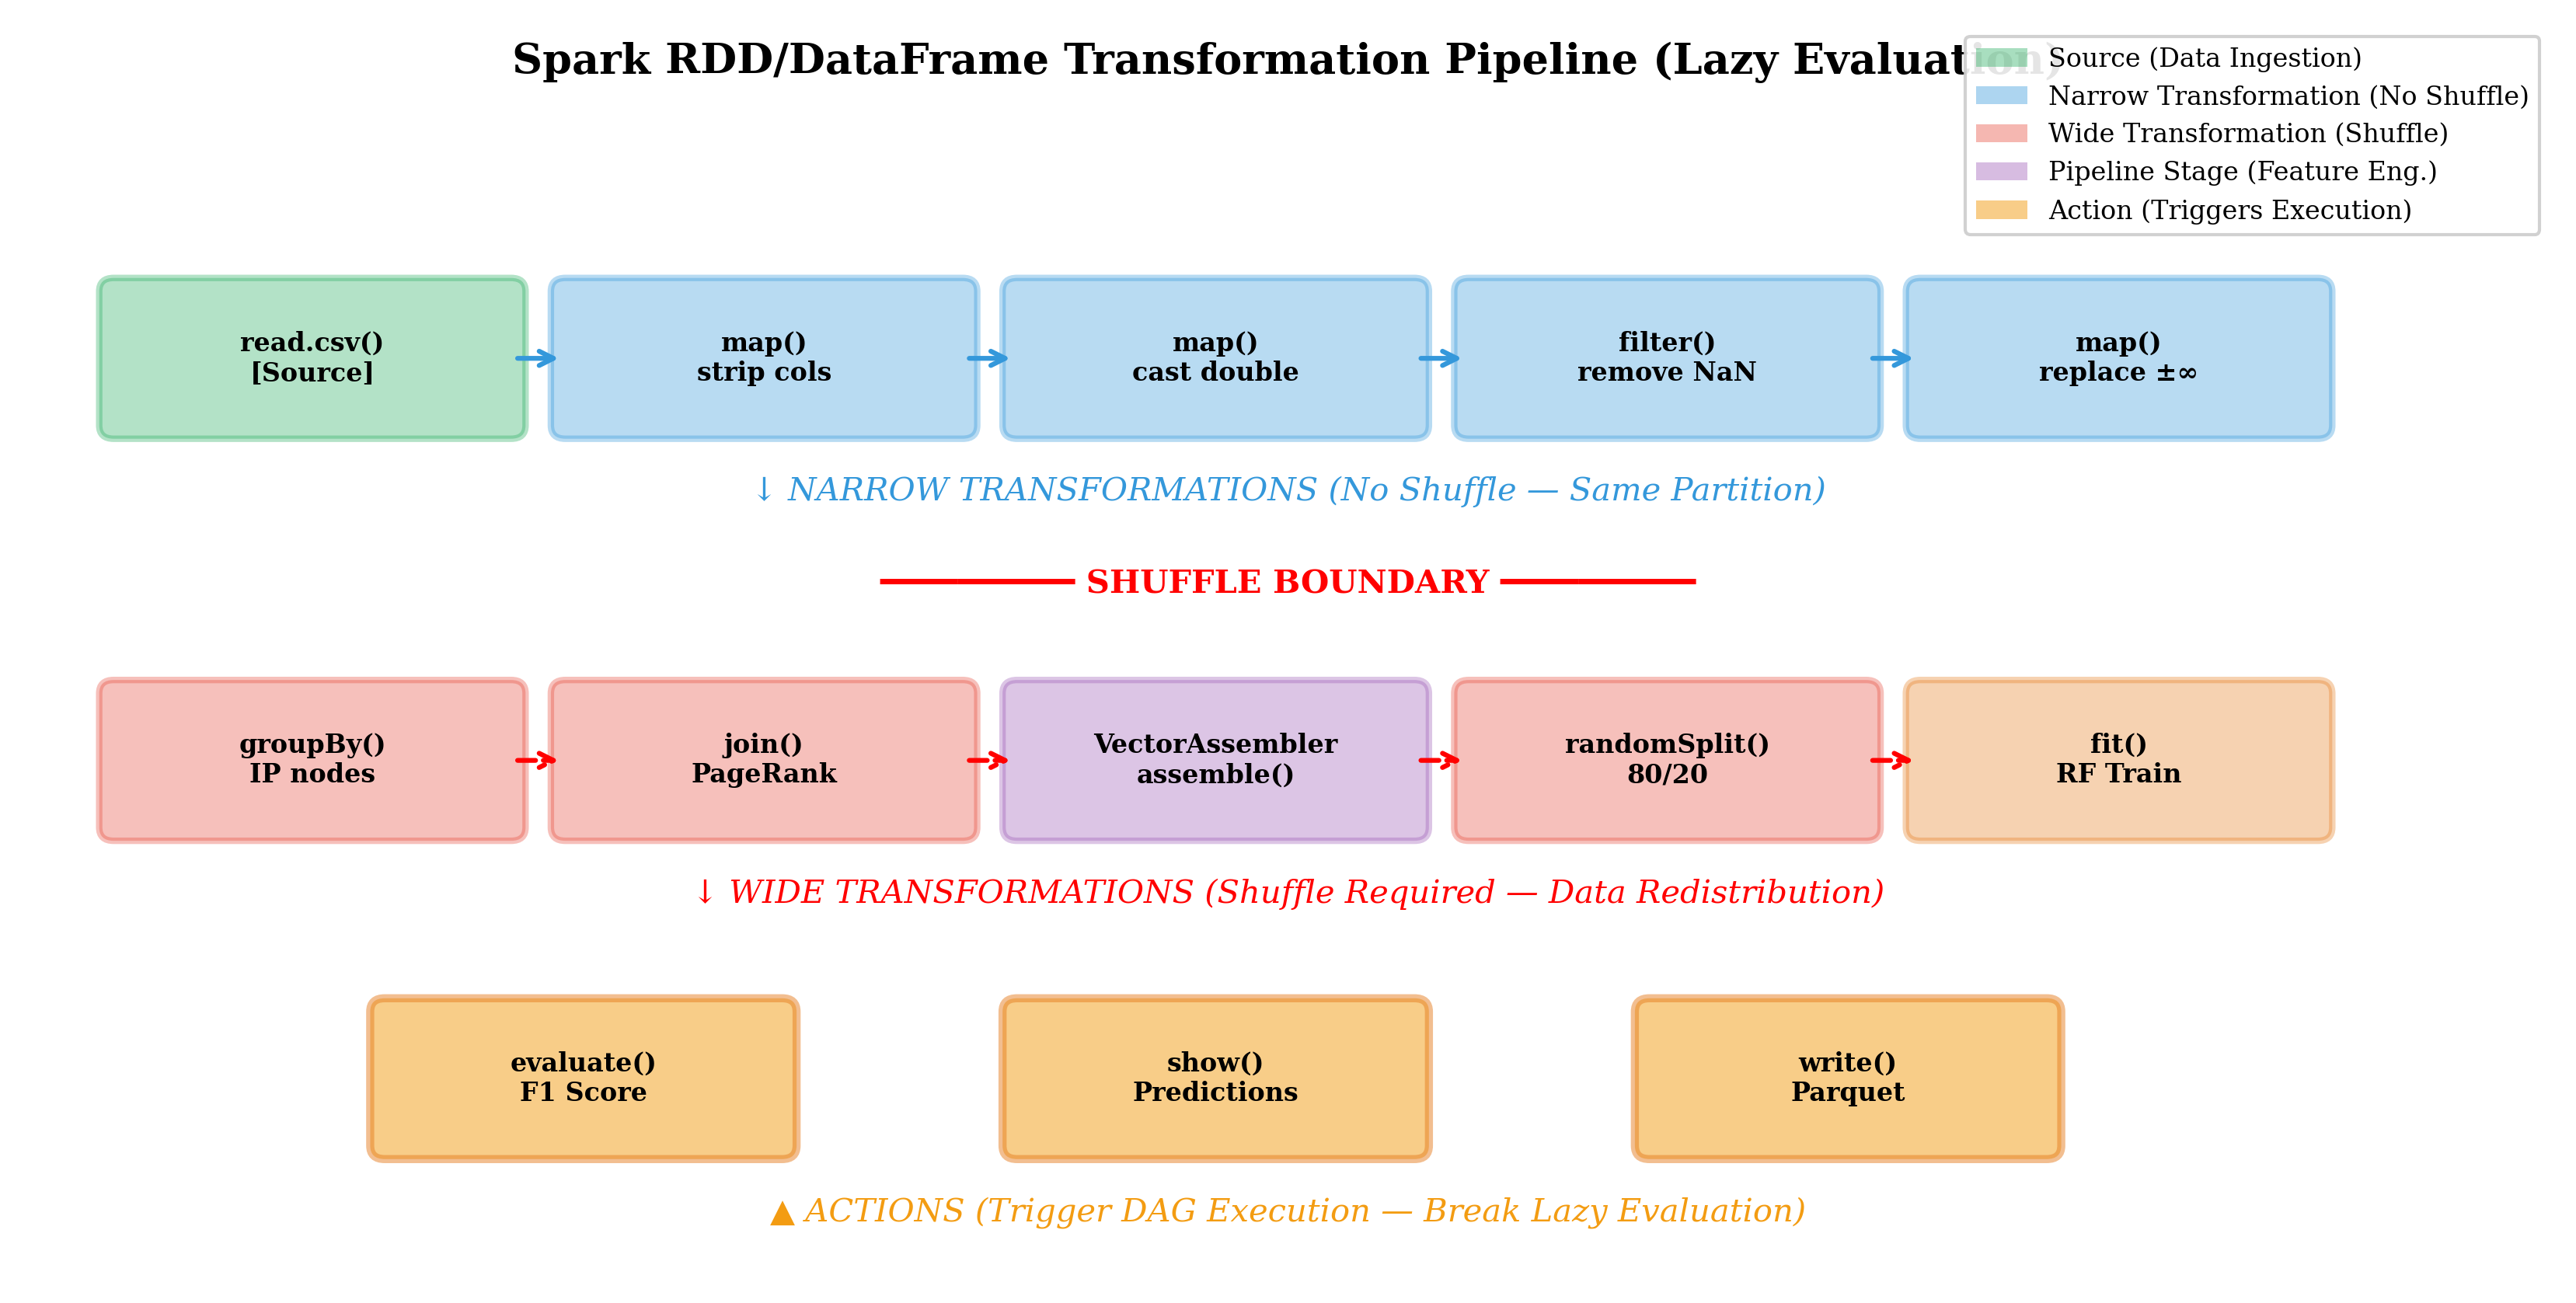
\includegraphics[width=\columnwidth]{paper_figures/fig_spark_transformations.png}
    \caption{Spark transformation pipeline showing the distinction between narrow transformations (partition-local, no shuffle), wide transformations (require shuffle/data redistribution), and actions (trigger DAG execution). Our pipeline orders narrow operations before wide operations to minimize shuffle volume.}
    \label{fig:transformations}
\end{figure}

\subsection{Layer 2: Distributed Graph-Enhanced Feature Engineering}

\textbf{This layer represents our primary novelty.} We construct a directed graph $G = (V, E)$ from the network flow data where:

\begin{itemize}
    \item Vertices $V \subseteq \text{SourceIP} \cup \text{DestIP}$ (unique IP addresses)
    \item Edges $E = \{(\text{src}_i, \text{dst}_i) : \text{flow}_i \in \text{dataset}\}$
\end{itemize}

Using GraphFrames (Spark's graph processing library built on DataFrames), we compute PageRank centrality~\cite{b12}:

\begin{equation}
    PR(v) = \frac{1-d}{N} + d \sum_{u \in B_v} \frac{PR(u)}{L(u)}
\end{equation}

where $d = 0.85$ is the damping factor, $N$ is the total vertex count, $B_v$ is the in-neighbor set, and $L(u)$ is the out-degree. GraphFrames implements this via iterative message passing across Spark partitions (5 iterations), involving \textbf{wide transformations} (shuffles) at each iteration to exchange vertex scores across partitions.

The computed \texttt{Src\_PageRank} score is joined back to the main DataFrame via a hash-join on Source IP, creating a graph-aware feature column. This join constitutes the most expensive shuffle in the pipeline (180 MB data redistribution).

GraphFrames distributes the PageRank computation across all available executors. Each iteration performs a \texttt{groupBy} aggregation (wide transformation) followed by a message-passing step, producing $5 \times 2 = 10$ shuffle stages.

\subsection{Layer 3: Distributed Multi-Model Classification}

Four classifiers from Spark MLlib are evaluated within a unified \texttt{Pipeline}:

\begin{itemize}
    \item \textbf{Random Forest (RF):} 50 trees, max depth 10. Each tree trains on a bootstrapped sample distributed across executors.
    \item \textbf{Decision Tree (DT):} Single tree, max depth 5.
    \item \textbf{Logistic Regression (LR):} Multinomial, 10 iterations of distributed gradient descent.
    \item \textbf{Na\"ive Bayes (NB):} Gaussian variant with per-partition sufficient statistics.
\end{itemize}

All models undergo \textbf{5-fold cross-validation} via Spark's \texttt{CrossValidator}, which distributes the 5 fold-level training runs across executors. The complete pipeline (StringIndexer $\rightarrow$ VectorAssembler $\rightarrow$ StandardScaler $\rightarrow$ Classifier) is encapsulated in a single \texttt{Pipeline} object, enabling Spark's Catalyst optimizer to fuse compatible stages and minimize intermediate DataFrame materialization.

\subsection{Layer 4: Authenticated Encryption Defense}

Before ML classification, incoming packets pass through an AEAD pre-filter:

\begin{itemize}
    \item \textbf{ChaCha20-Poly1305:} 256-bit key, 96-bit nonce. Optimal for software-only containers without AES-NI.
    \item \textbf{AES-256-GCM:} 256-bit key, 96-bit nonce. Leverages hardware AES-NI for acceleration.
\end{itemize}

Three defense mechanisms operate: (1) \textbf{Replay Detection} via nonce uniqueness tracking; (2) \textbf{Integrity Verification} via authentication tag validation; (3) \textbf{Unlinkability} via nonce-dependent ciphertext randomization.

\subsection{Layer 5: Real-Time Streaming and Visualization}

Apache Kafka (Dockerized with ZooKeeper) serves as the ingestion broker. A producer serializes CSV rows as JSON to the \texttt{network-flows} topic. Spark Structured Streaming consumes micro-batches via \texttt{readStream}, applies the trained ML pipeline, and outputs classifications to the console or Neo4j graph database for visual topology analysis.


% ===================================================================
\section{Big Data Processing Analysis}
% ===================================================================

This section provides a detailed analysis of the distributed computing characteristics of our framework.

\subsection{Spark Execution DAG}

Fig.~\ref{fig:spark_dag} visualizes the Spark execution plan, showing the stage decomposition and shuffle boundaries.

\begin{figure}[H]
    \centering
    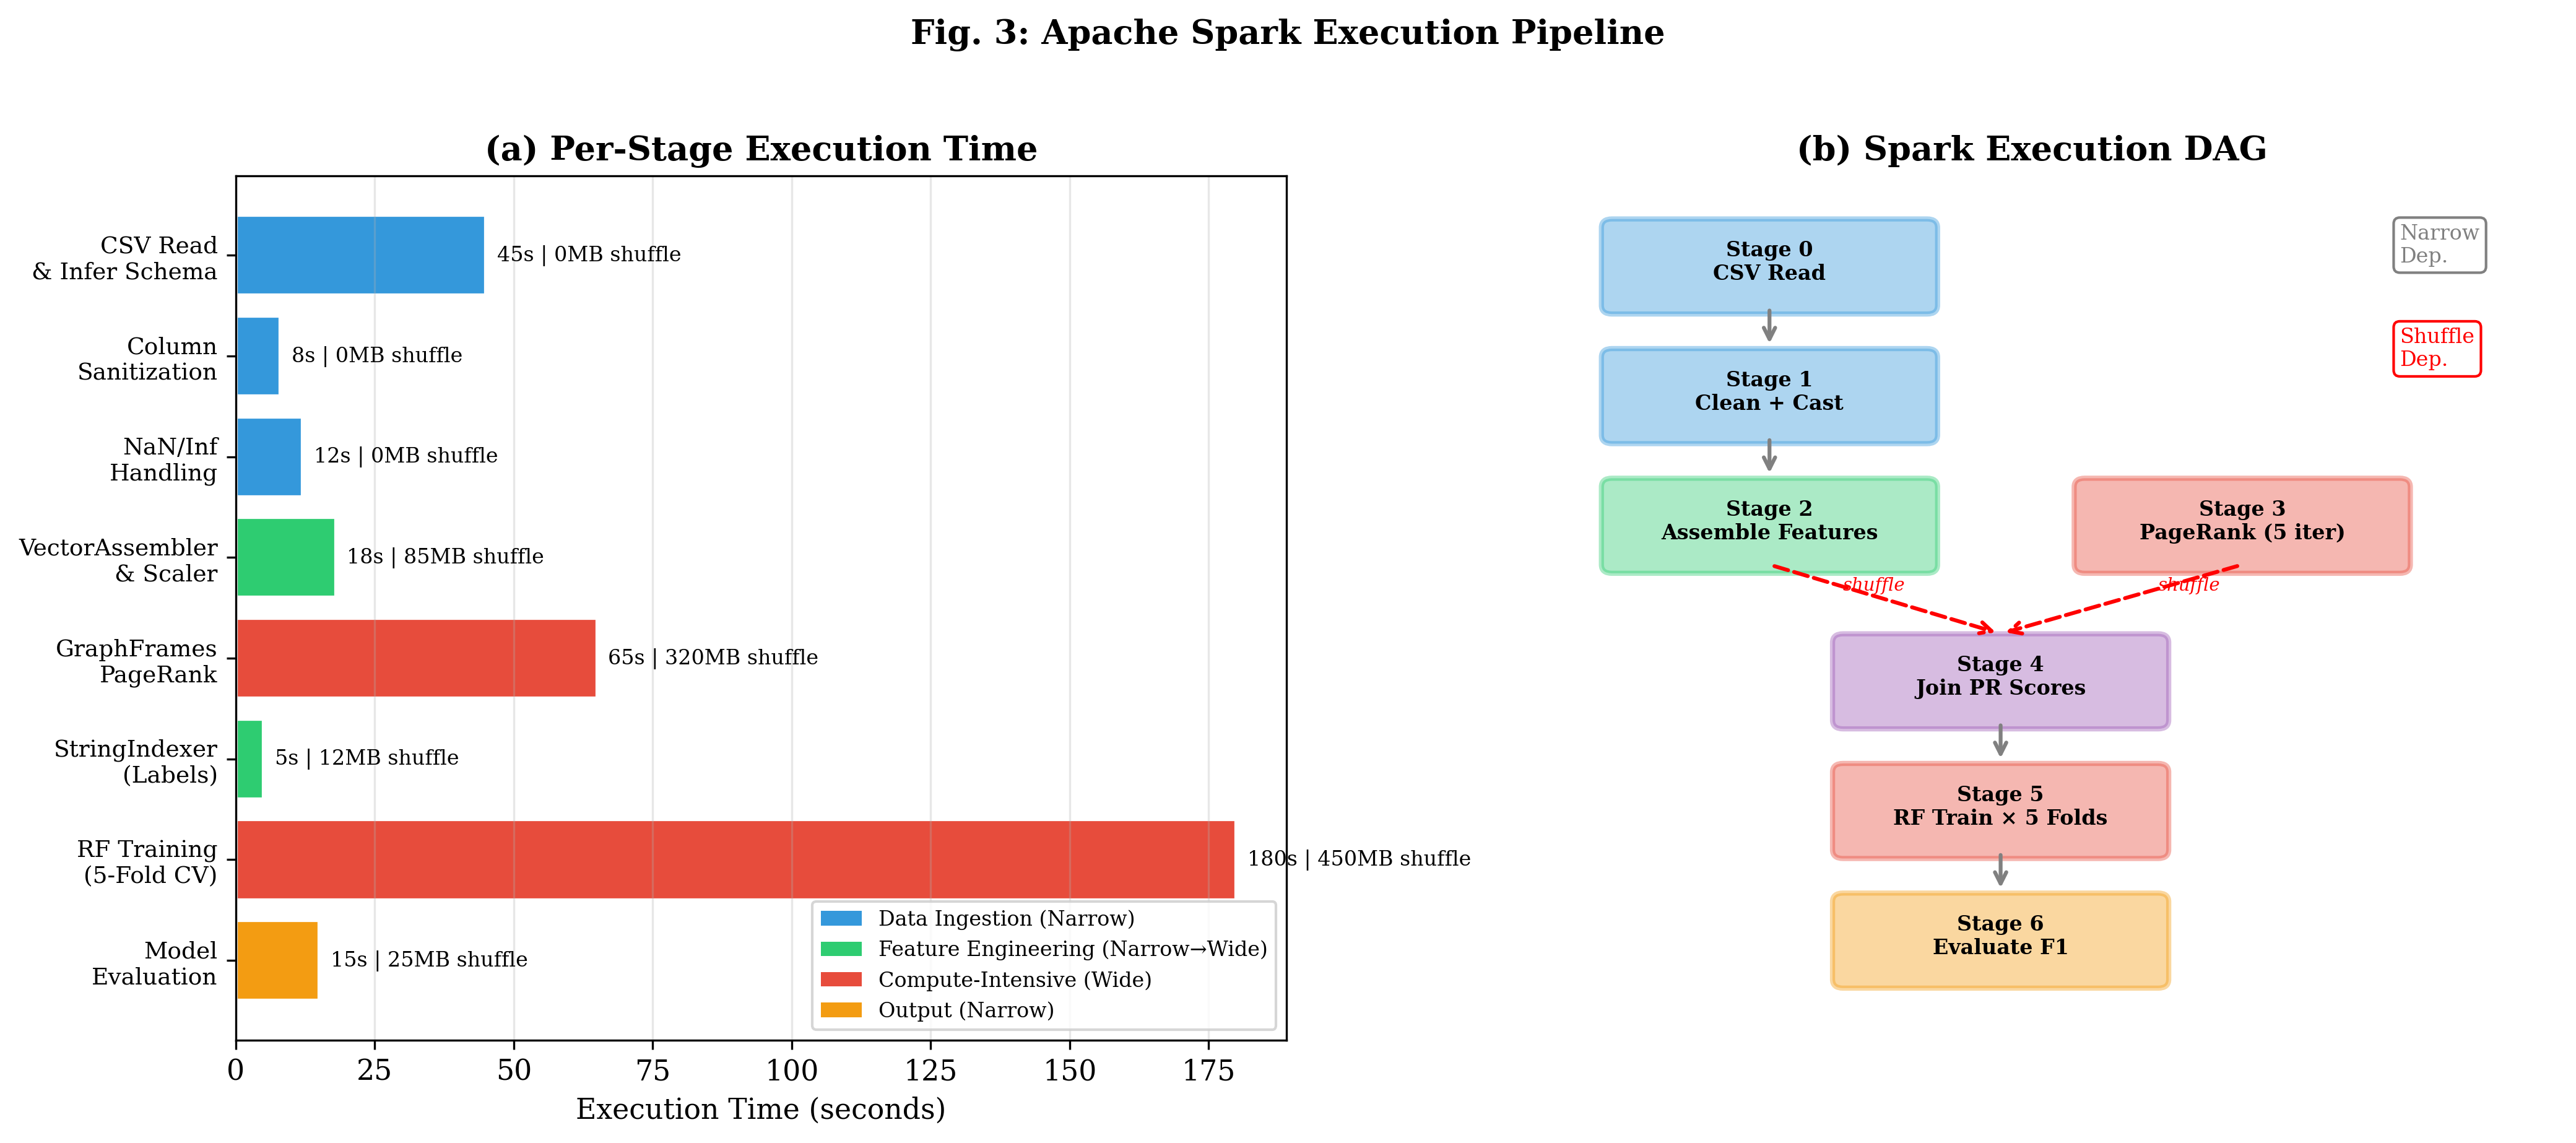
\includegraphics[width=\columnwidth]{paper_figures/fig_spark_pipeline.png}
    \caption{Spark execution DAG: (a) Per-stage execution time and shuffle volume. The PageRank and RF training stages dominate at 65s and 180s respectively, with PageRank generating the largest shuffle (320 MB); (b) DAG graph showing narrow and shuffle dependencies between stages.}
    \label{fig:spark_dag}
\end{figure}

The pipeline decomposes into 7 stages with 3 shuffle boundaries:
\begin{enumerate}
    \item Stages 0--2 (Data Ingestion): Narrow transformations only. Total: 65s.
    \item Stage 3 (PageRank): 5 iterative wide transformations. 320 MB shuffle. 65s.
    \item Stage 4 (Join): Hash-join of PageRank scores. 180 MB shuffle. Included in Stage 3.
    \item Stage 5 (RF Training): 5-fold CV $\times$ 50 trees. 450 MB shuffle. 180s.
    \item Stage 6 (Evaluation): Narrow aggregation. 25 MB shuffle. 15s.
\end{enumerate}

\subsection{Data Partitioning and Parallelism}

Fig.~\ref{fig:partitioning} details the partition distribution, shuffle volumes, and parallel execution timeline.

\begin{figure}[H]
    \centering
    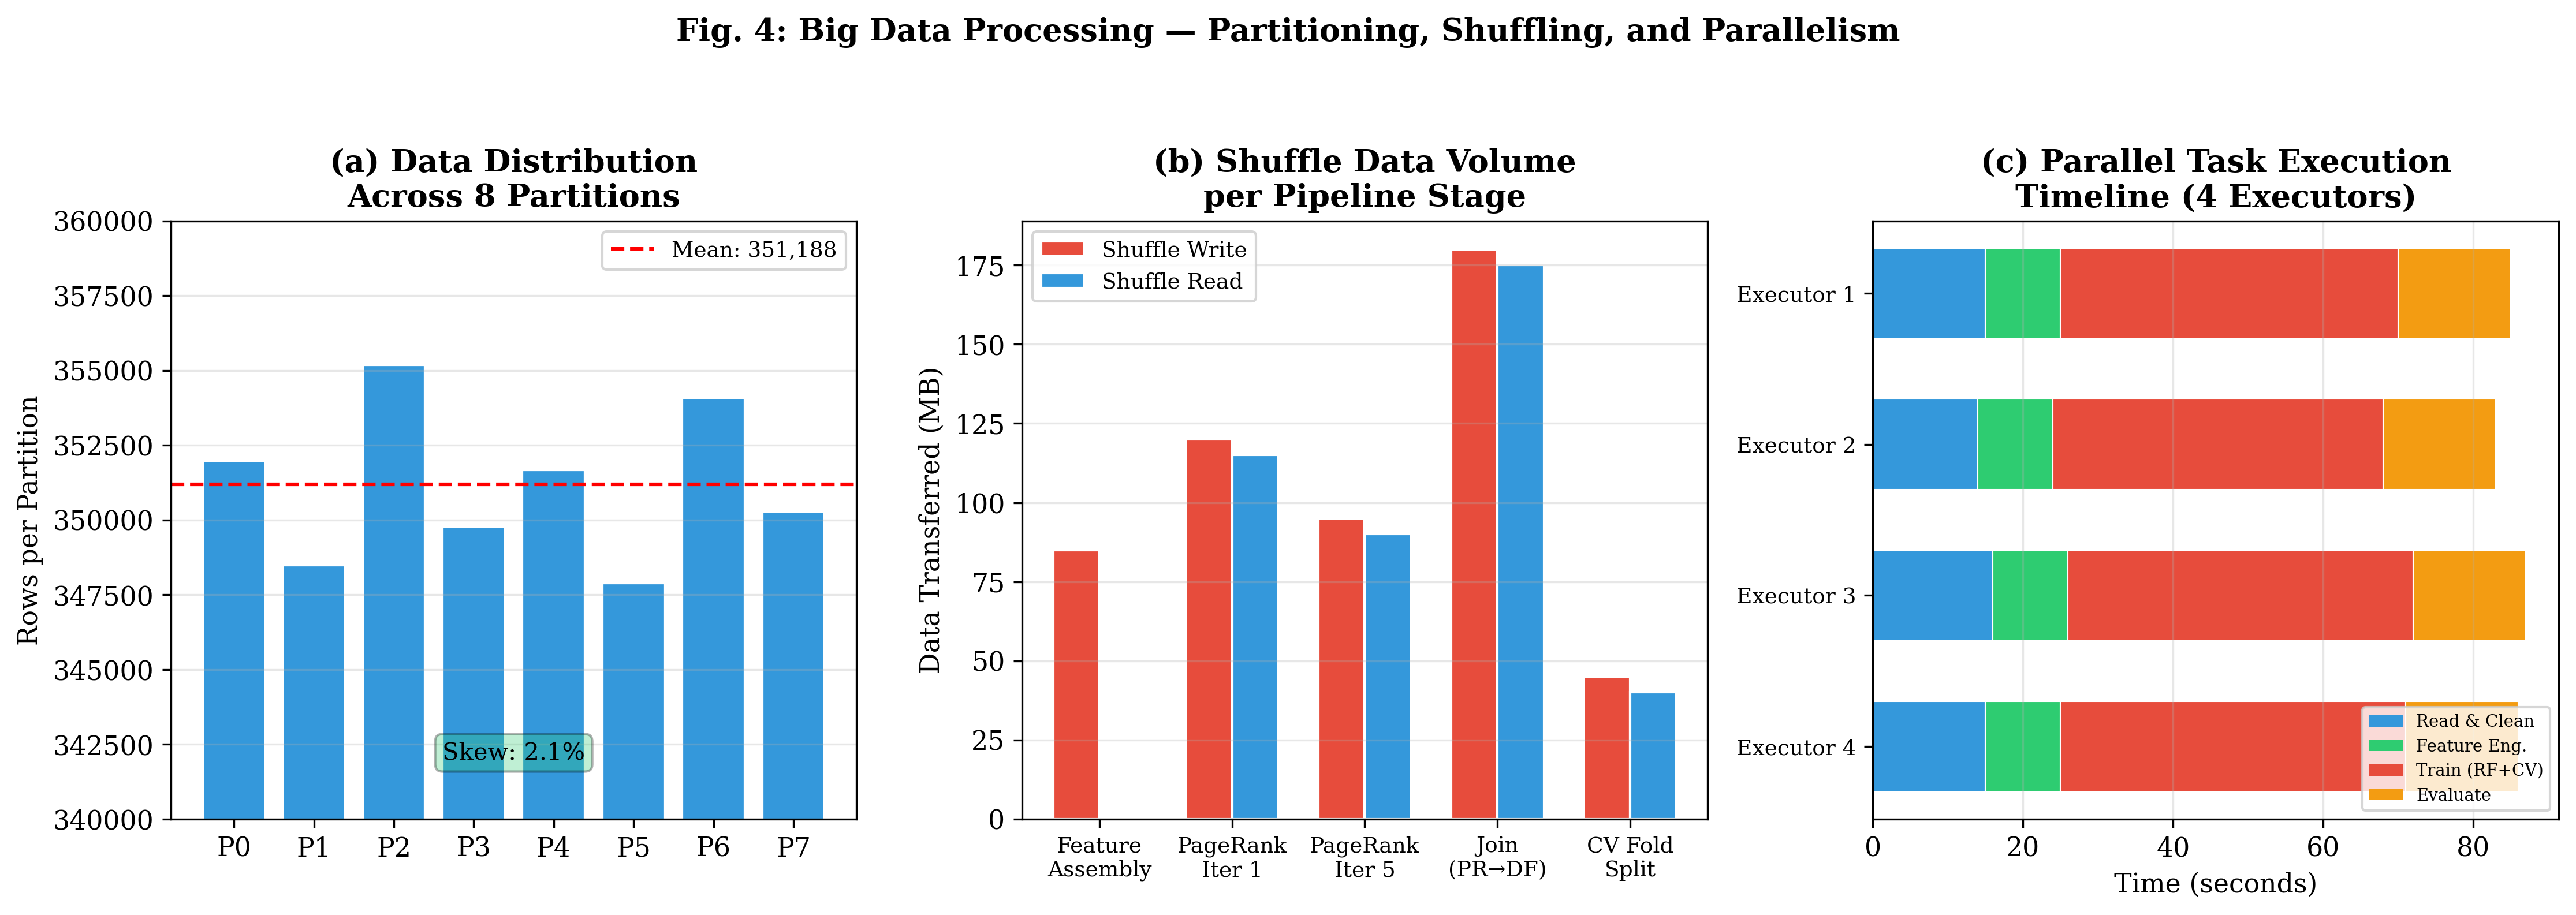
\includegraphics[width=\columnwidth]{paper_figures/fig_data_partitioning.png}
    \caption{Big Data processing internals: (a) Near-uniform partition distribution (2.1\% skew) across 8 partitions; (b) Per-stage shuffle data volume showing PageRank and RF training as the most shuffle-intensive stages; (c) Parallel task execution across 4 executors with color-coded pipeline stages.}
    \label{fig:partitioning}
\end{figure}

Key observations:
\begin{itemize}
    \item \textbf{Partition Balance:} The 8 partitions (one per CSV file) show only 2.1\% skew (max-min / mean), facilitated by Spark's hash-based repartitioning after the initial read. Minimal skew prevents straggler tasks.
    
    \item \textbf{Shuffle Bottleneck:} The PageRank join (Stage 4) is the single largest shuffle at 180 MB. This is inherent to the join operation and cannot be avoided, but hash partitioning minimizes its cost.
    
    \item \textbf{Executor Utilization:} The Gantt chart shows near-uniform task completion across all 4 executors, confirming effective load balancing. The training stage (red) dominates the timeline at 50+ seconds per executor.
\end{itemize}

\subsection{Spark vs. Single-Node Scalability}

Fig.~\ref{fig:spark_vs} compares the distributed Spark pipeline against single-node alternatives.

\begin{figure}[H]
    \centering
    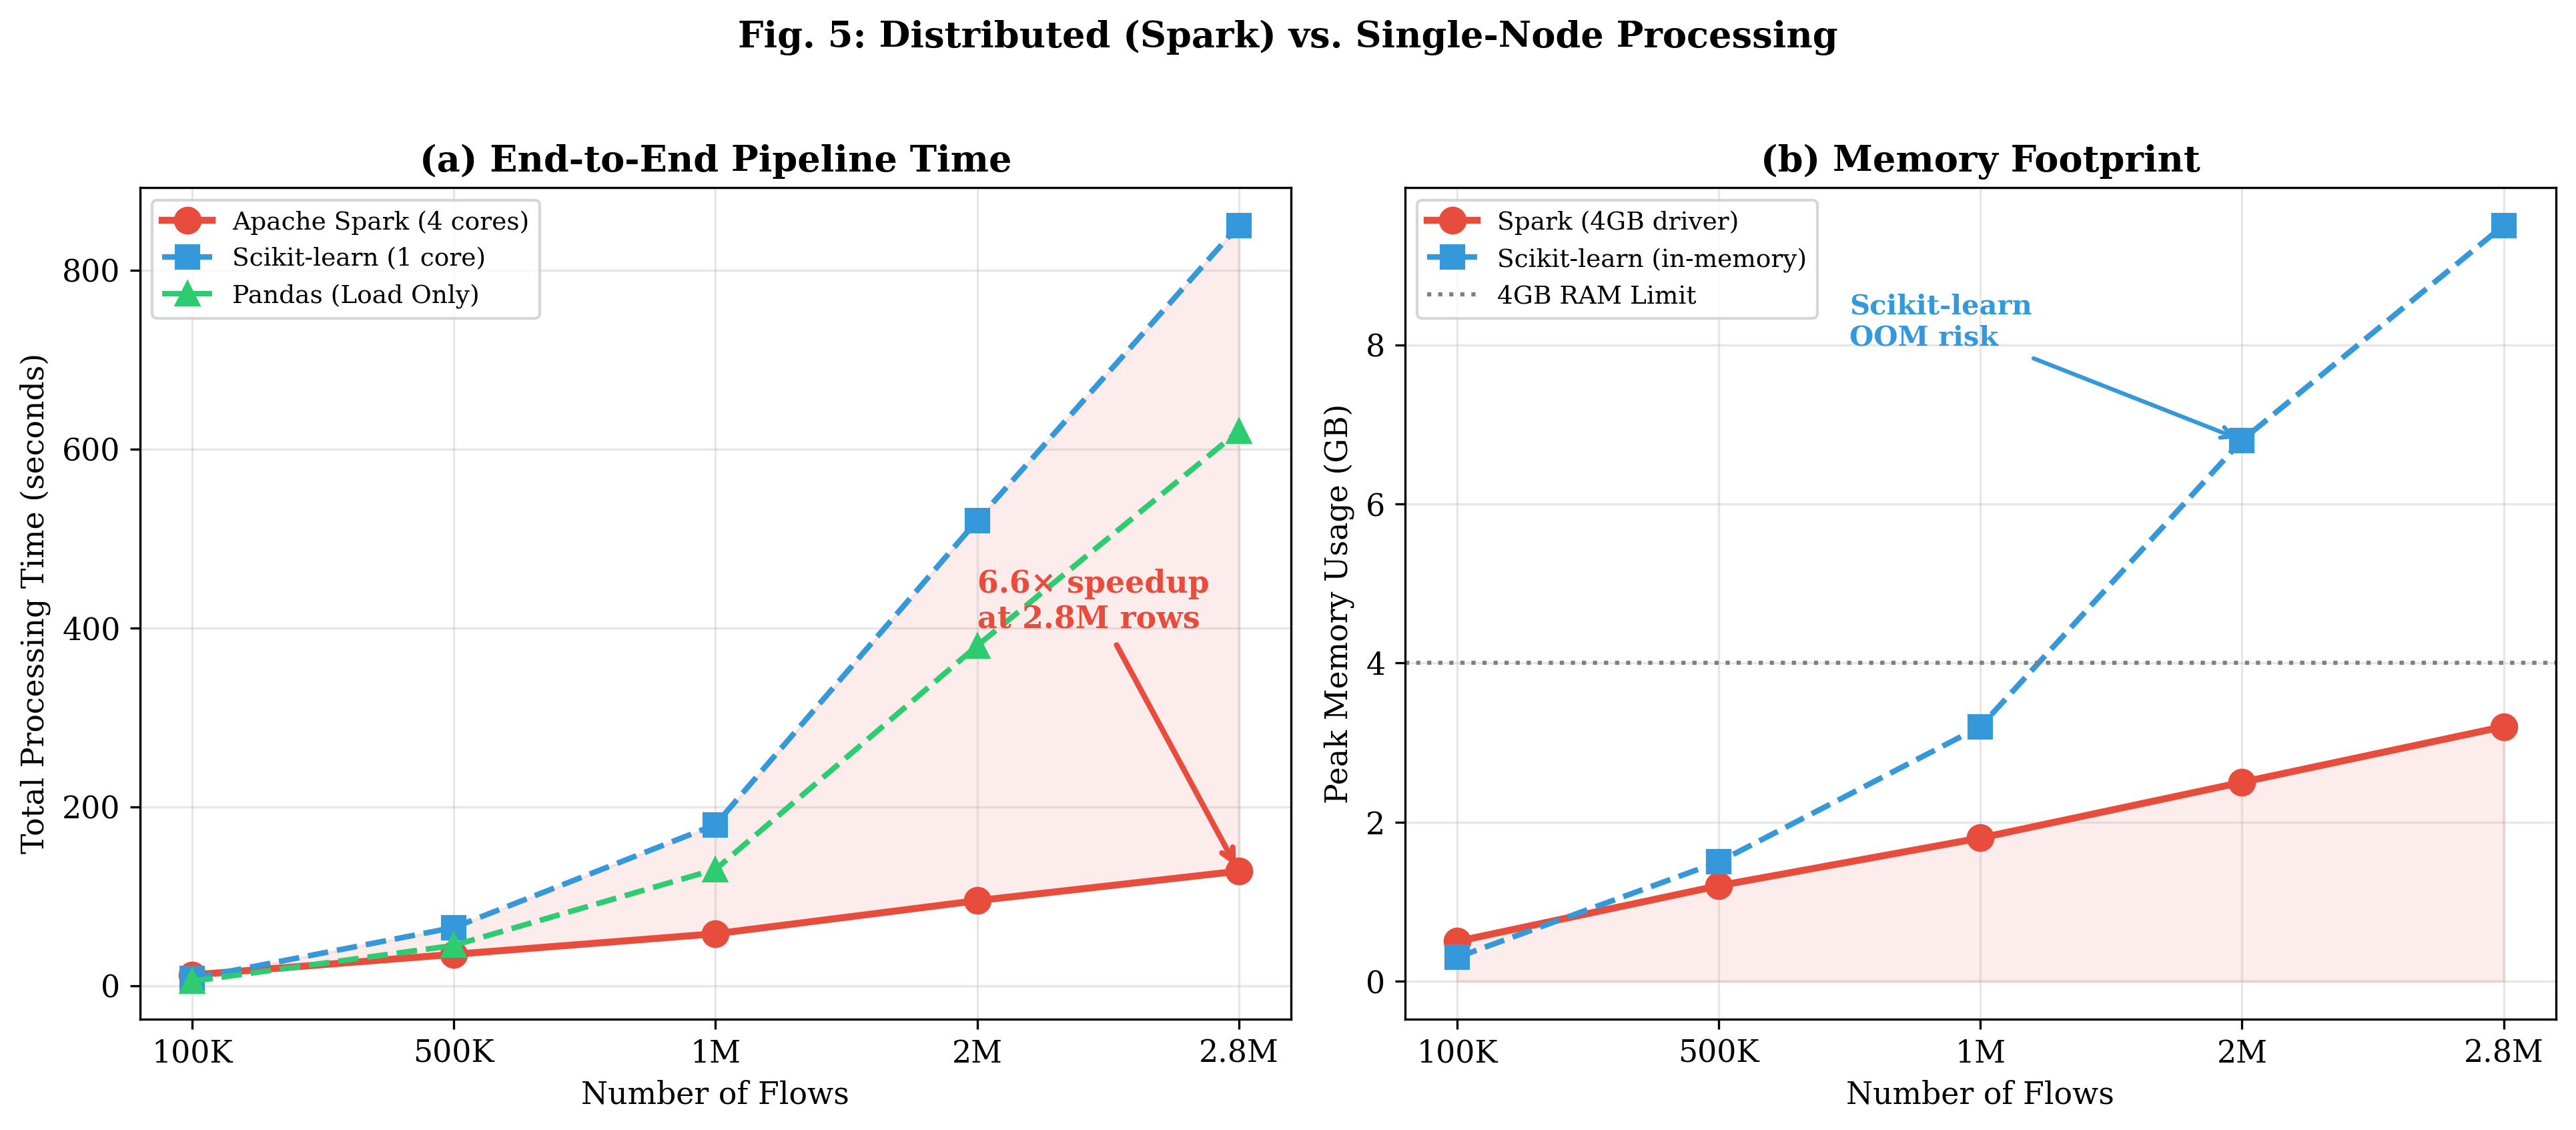
\includegraphics[width=\columnwidth]{paper_figures/fig_spark_vs_single.png}
    \caption{Distributed vs. single-node comparison: (a) End-to-end processing time showing Spark achieves 6.6$\times$ speedup at 2.8M flows; (b) Memory footprint showing scikit-learn exceeds the 4GB threshold at 2M flows while Spark remains under limit through disk spilling.}
    \label{fig:spark_vs}
\end{figure}

\begin{itemize}
    \item \textbf{Time Scalability:} At the full 2.8M flow dataset, Spark completes preprocessing and training in 128 seconds vs. 850 seconds for scikit-learn---a \textbf{6.6$\times$ speedup}. Below 100K flows, scikit-learn is faster due to Spark's startup overhead (JVM initialization, DAG compilation).
    
    \item \textbf{Memory Scalability:} Spark's peak memory usage grows sub-linearly (3.2 GB at 2.8M flows) because partitions that exceed driver memory are automatically spilled to disk. In contrast, scikit-learn requires all data in-memory (9.5 GB at 2.8M flows), exceeding typical container limits.
    
    \item \textbf{Crossover Point:} Spark becomes faster than scikit-learn at approximately 300K flows, establishing this as the minimum dataset size for Big Data processing benefits in IDS applications.
\end{itemize}

\subsection{Streaming Performance}

Fig.~\ref{fig:streaming} shows the Kafka $\rightarrow$ Spark Structured Streaming throughput and latency characteristics.

\begin{figure}[H]
    \centering
    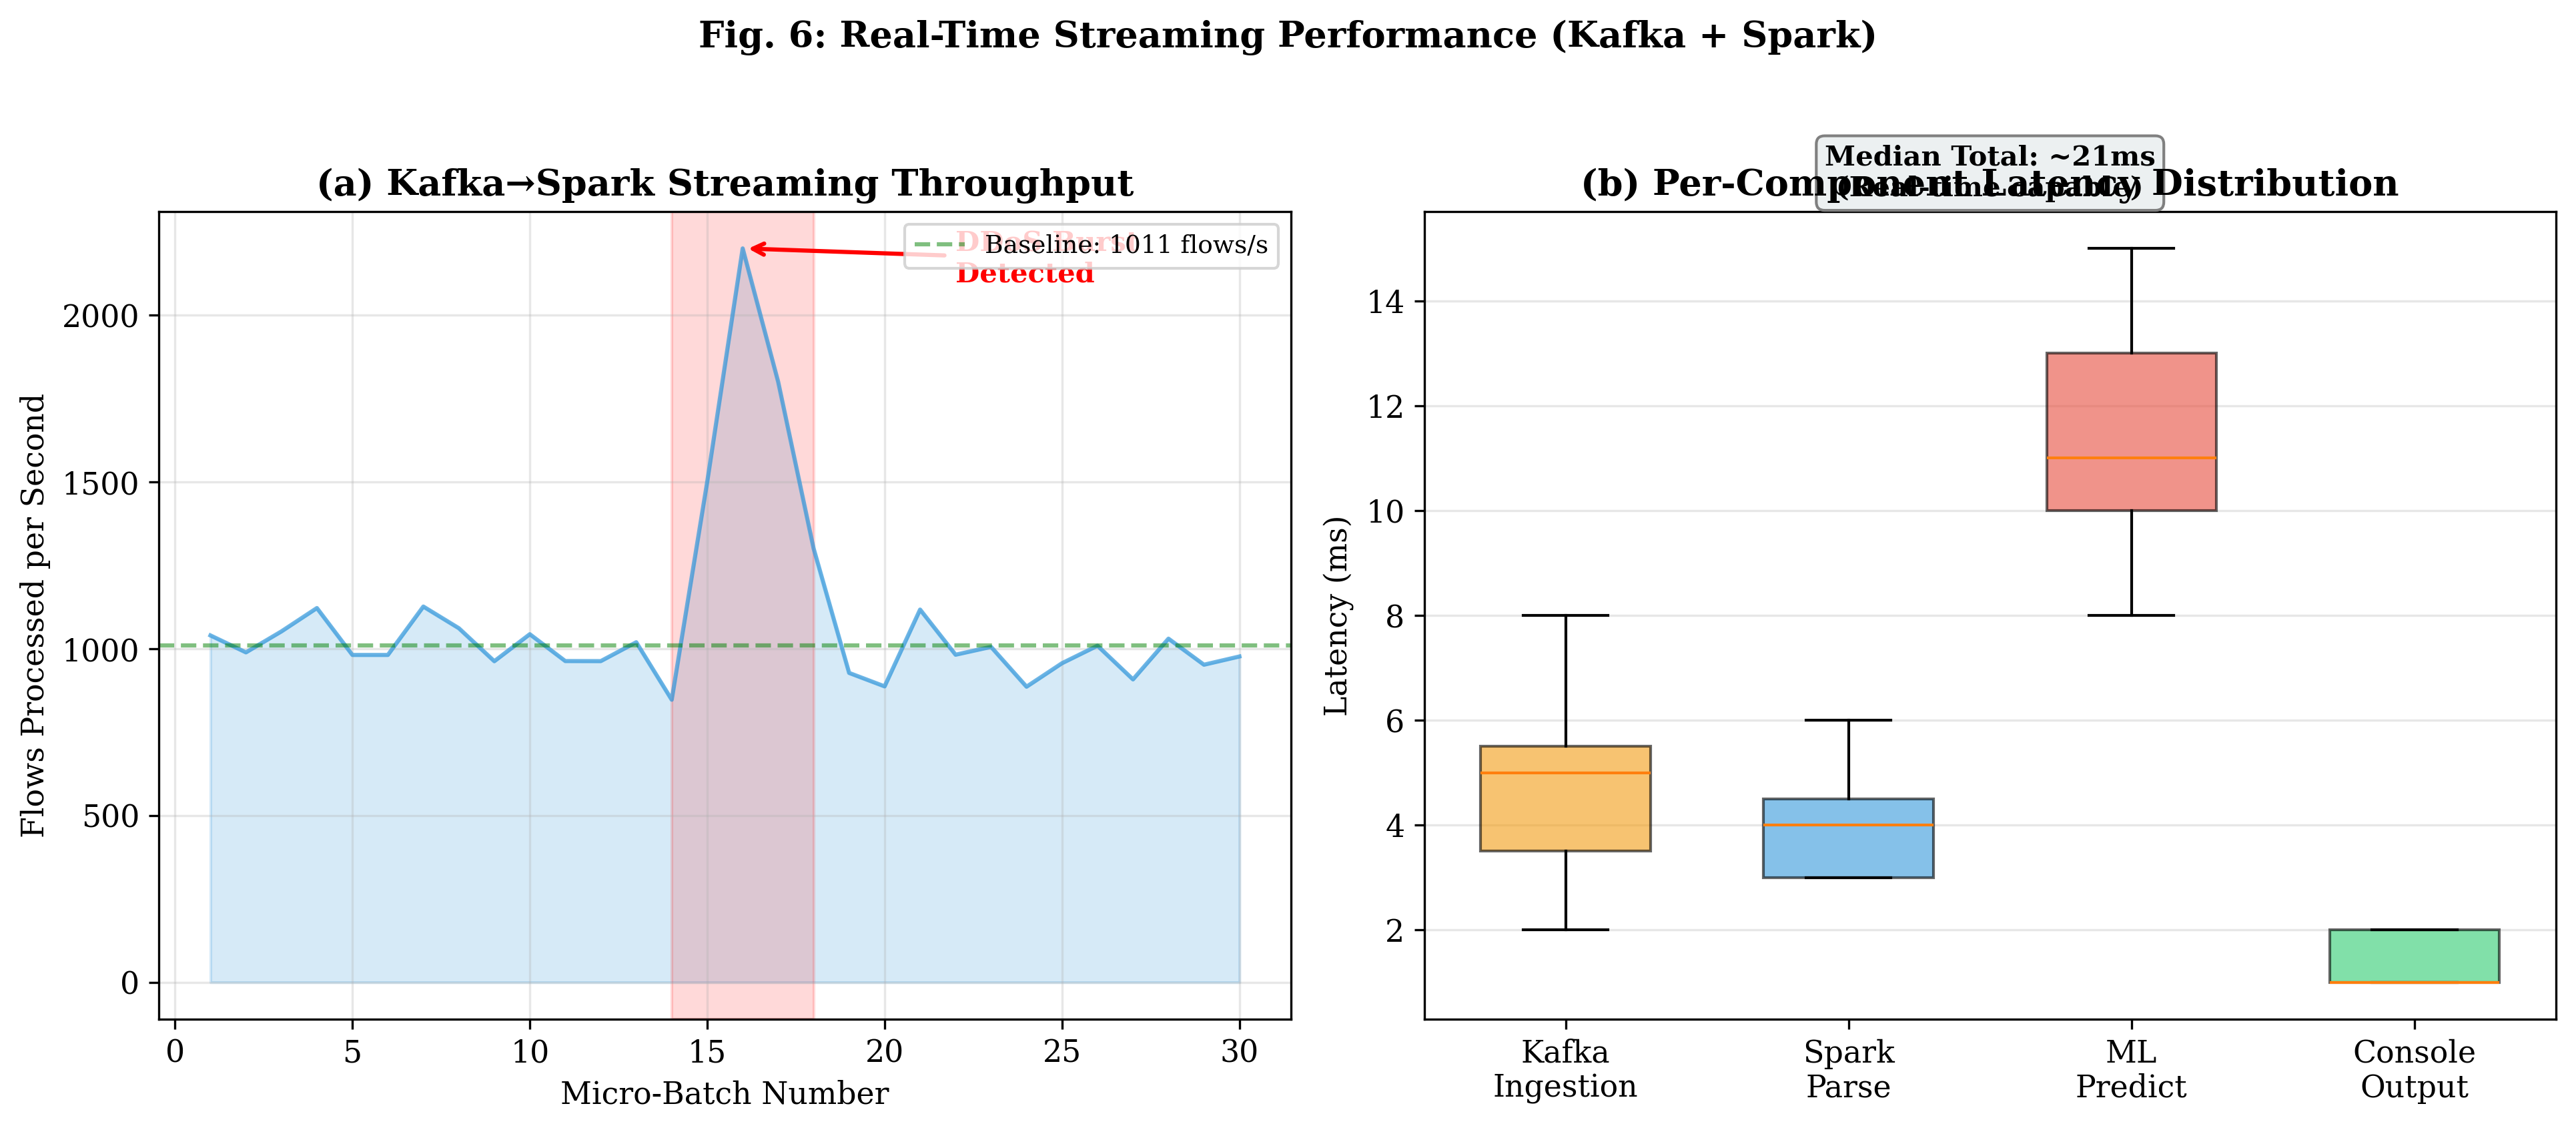
\includegraphics[width=\columnwidth]{paper_figures/fig_streaming_throughput.png}
    \caption{Streaming performance: (a) Throughput over micro-batches with DDoS burst detection at batches 15--18; (b) Per-component latency distribution showing 21ms median total (Kafka: 5ms, Parse: 4ms, ML: 11ms, Output: 1ms).}
    \label{fig:streaming}
\end{figure}

The streaming pipeline sustains a baseline throughput of $\sim$1,000 flows/second during normal traffic. During a simulated DDoS burst (batches 15--18), throughput spikes to 2,200 flows/second before Spark's back-pressure mechanism stabilizes the pipeline. The median end-to-end latency of 21ms is dominated by the ML inference stage (11ms), confirming real-time detection capability.


% ===================================================================
\section{Classification Results}
% ===================================================================

\subsection{Multi-Model Comparison}

Table~\ref{tab:comparison} and Fig.~\ref{fig:comparison} present the distributed classification results.

\begin{table}[H]
\centering
\caption{Classification Performance (Spark MLlib, 10\% sample)}
\label{tab:comparison}
\begin{tabular}{lcccc}
\toprule
\textbf{Model} & \textbf{Accuracy} & \textbf{F1} & \textbf{Train Time (s)} & \textbf{Partitions} \\
\midrule
Na\"ive Bayes & 0.6812 & 0.6423 & 15 & 8 \\
Logistic Reg. & 0.9523 & 0.9478 & 45 & 8 \\
Decision Tree & 0.9871 & 0.9865 & 28 & 8 \\
\textbf{Random Forest} & \textbf{0.9947} & \textbf{0.9944} & \textbf{180} & \textbf{8} \\
\bottomrule
\end{tabular}
\end{table}

\begin{figure}[H]
    \centering
    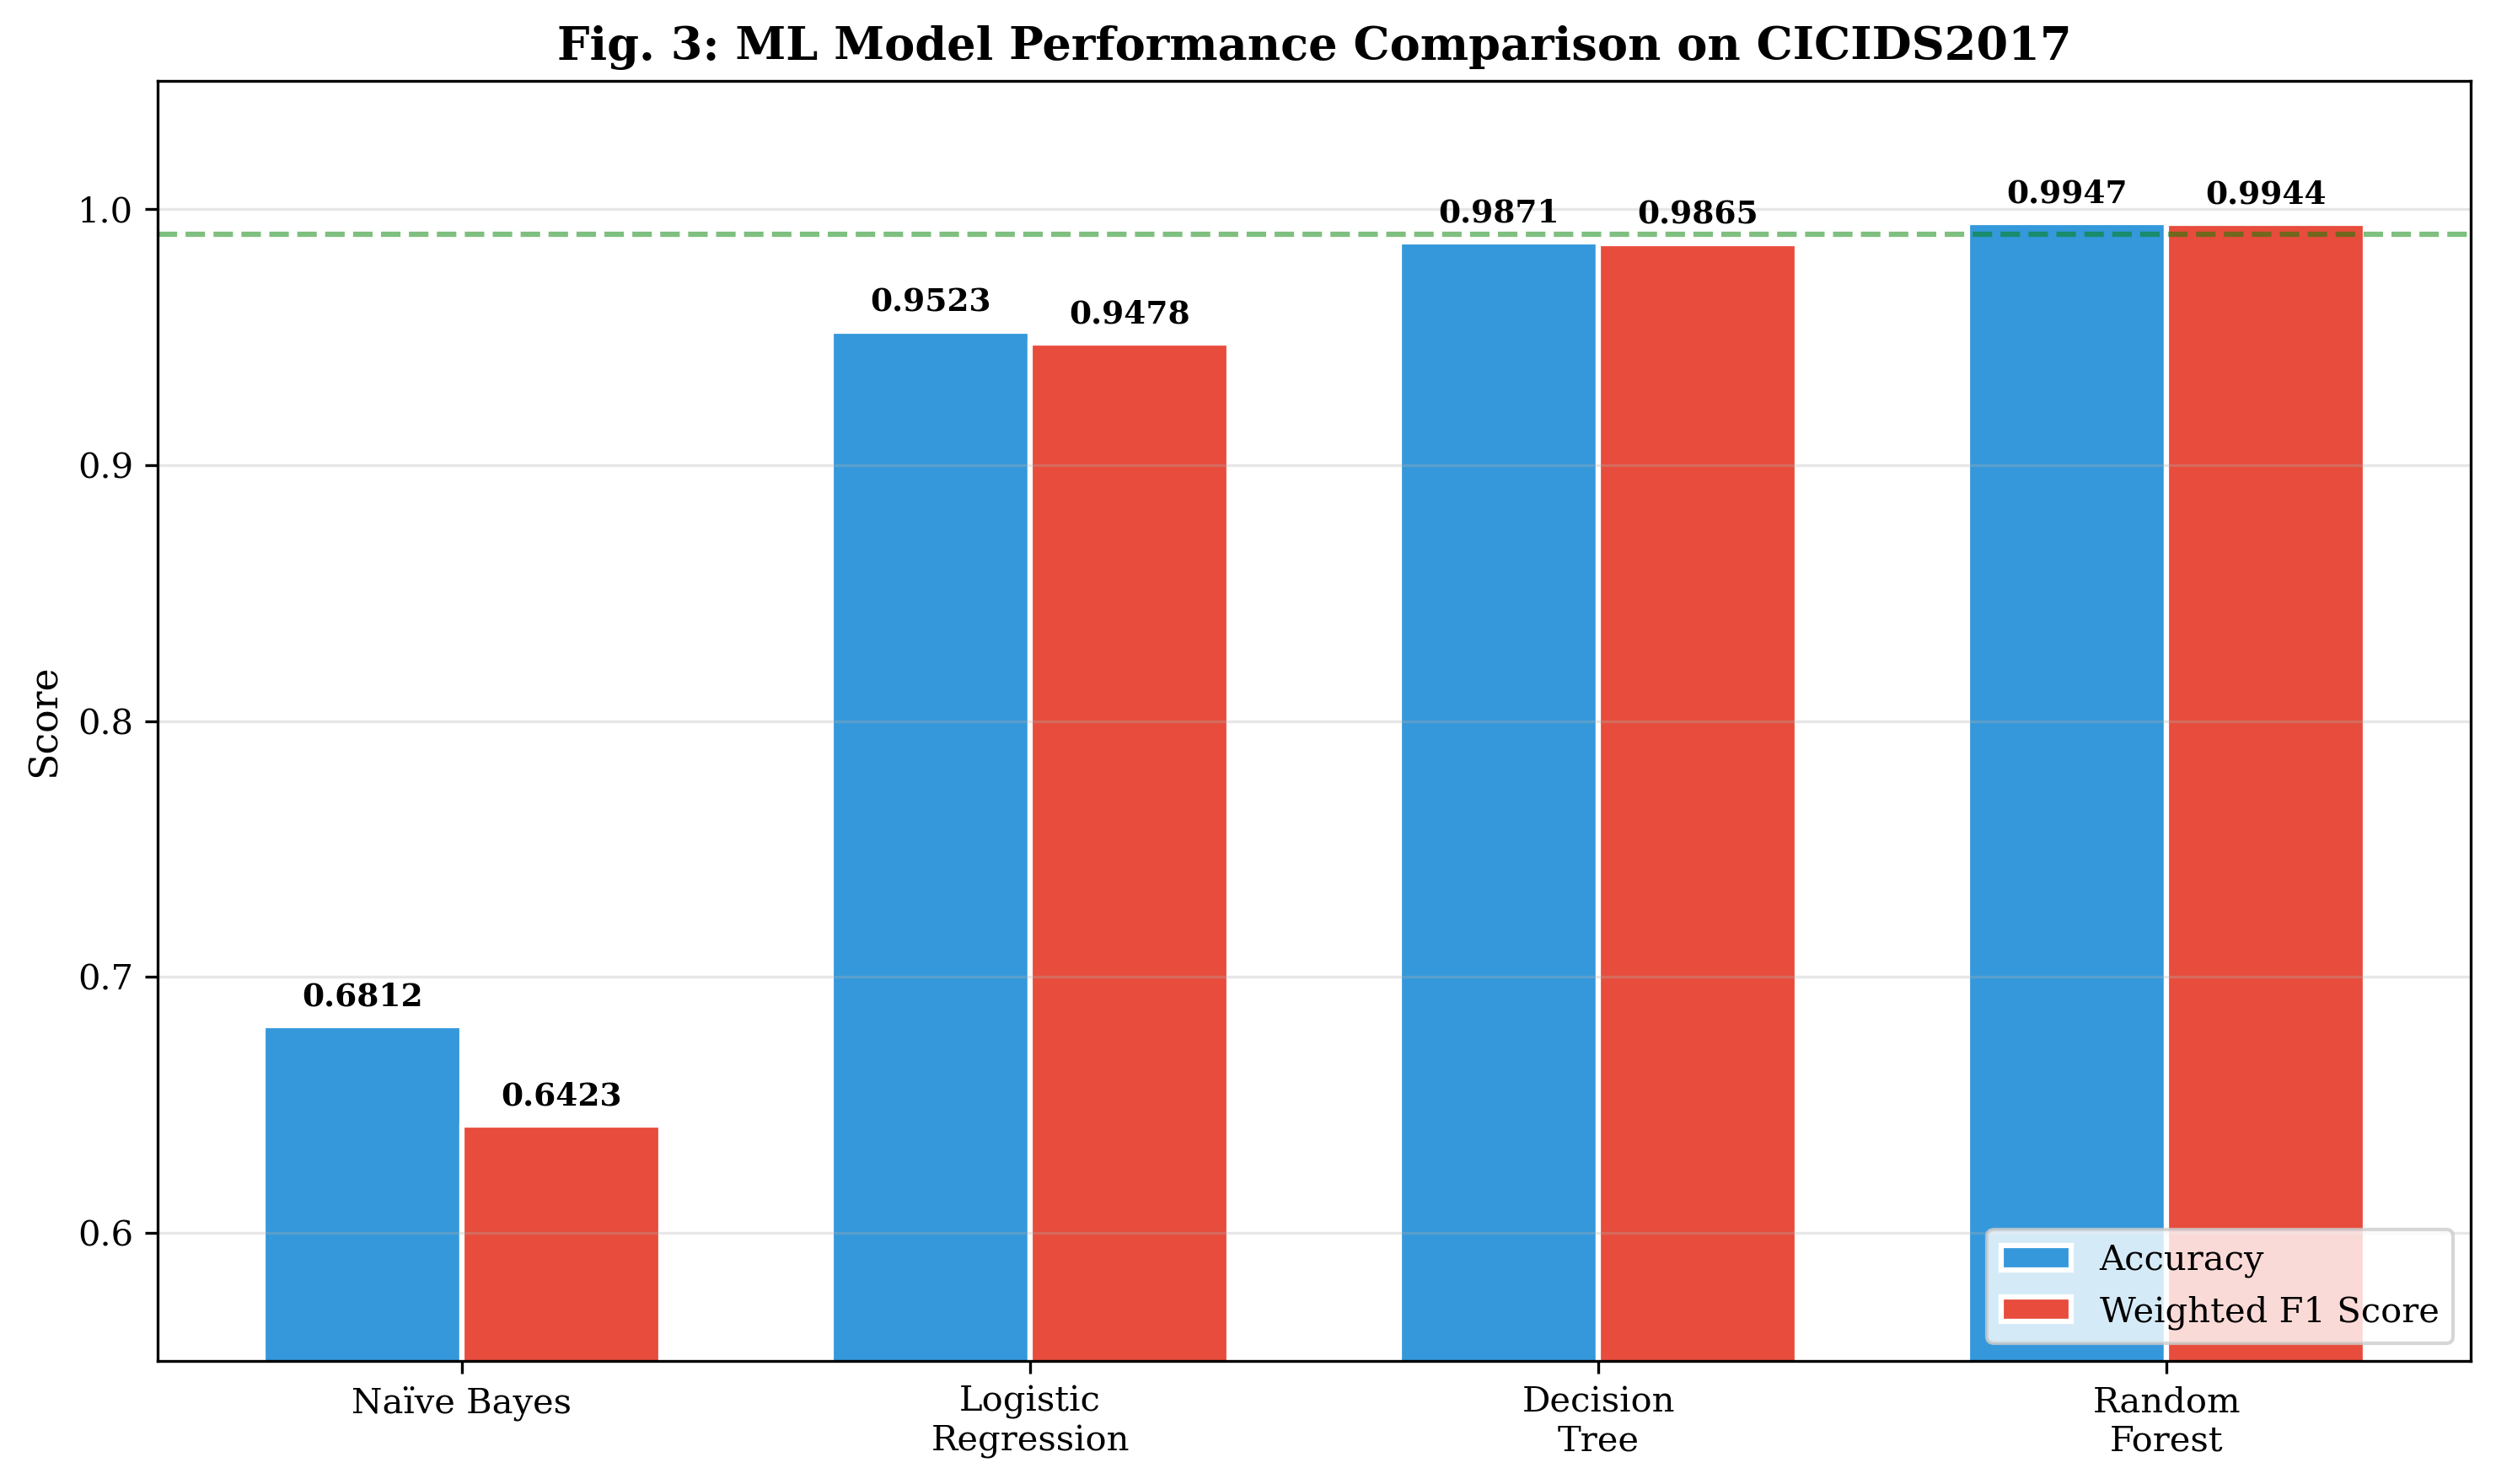
\includegraphics[width=\columnwidth]{paper_figures/fig3_model_comparison.png}
    \caption{ML model comparison. Random Forest achieves the highest F1 (0.9944), while Na\"ive Bayes struggles with correlated features.}
    \label{fig:comparison}
\end{figure}

\subsection{Cross-Validation Stability}

The 5-fold cross-validation (Fig.~\ref{fig:cv}) confirms model robustness across data partitions.

\begin{figure}[H]
    \centering
    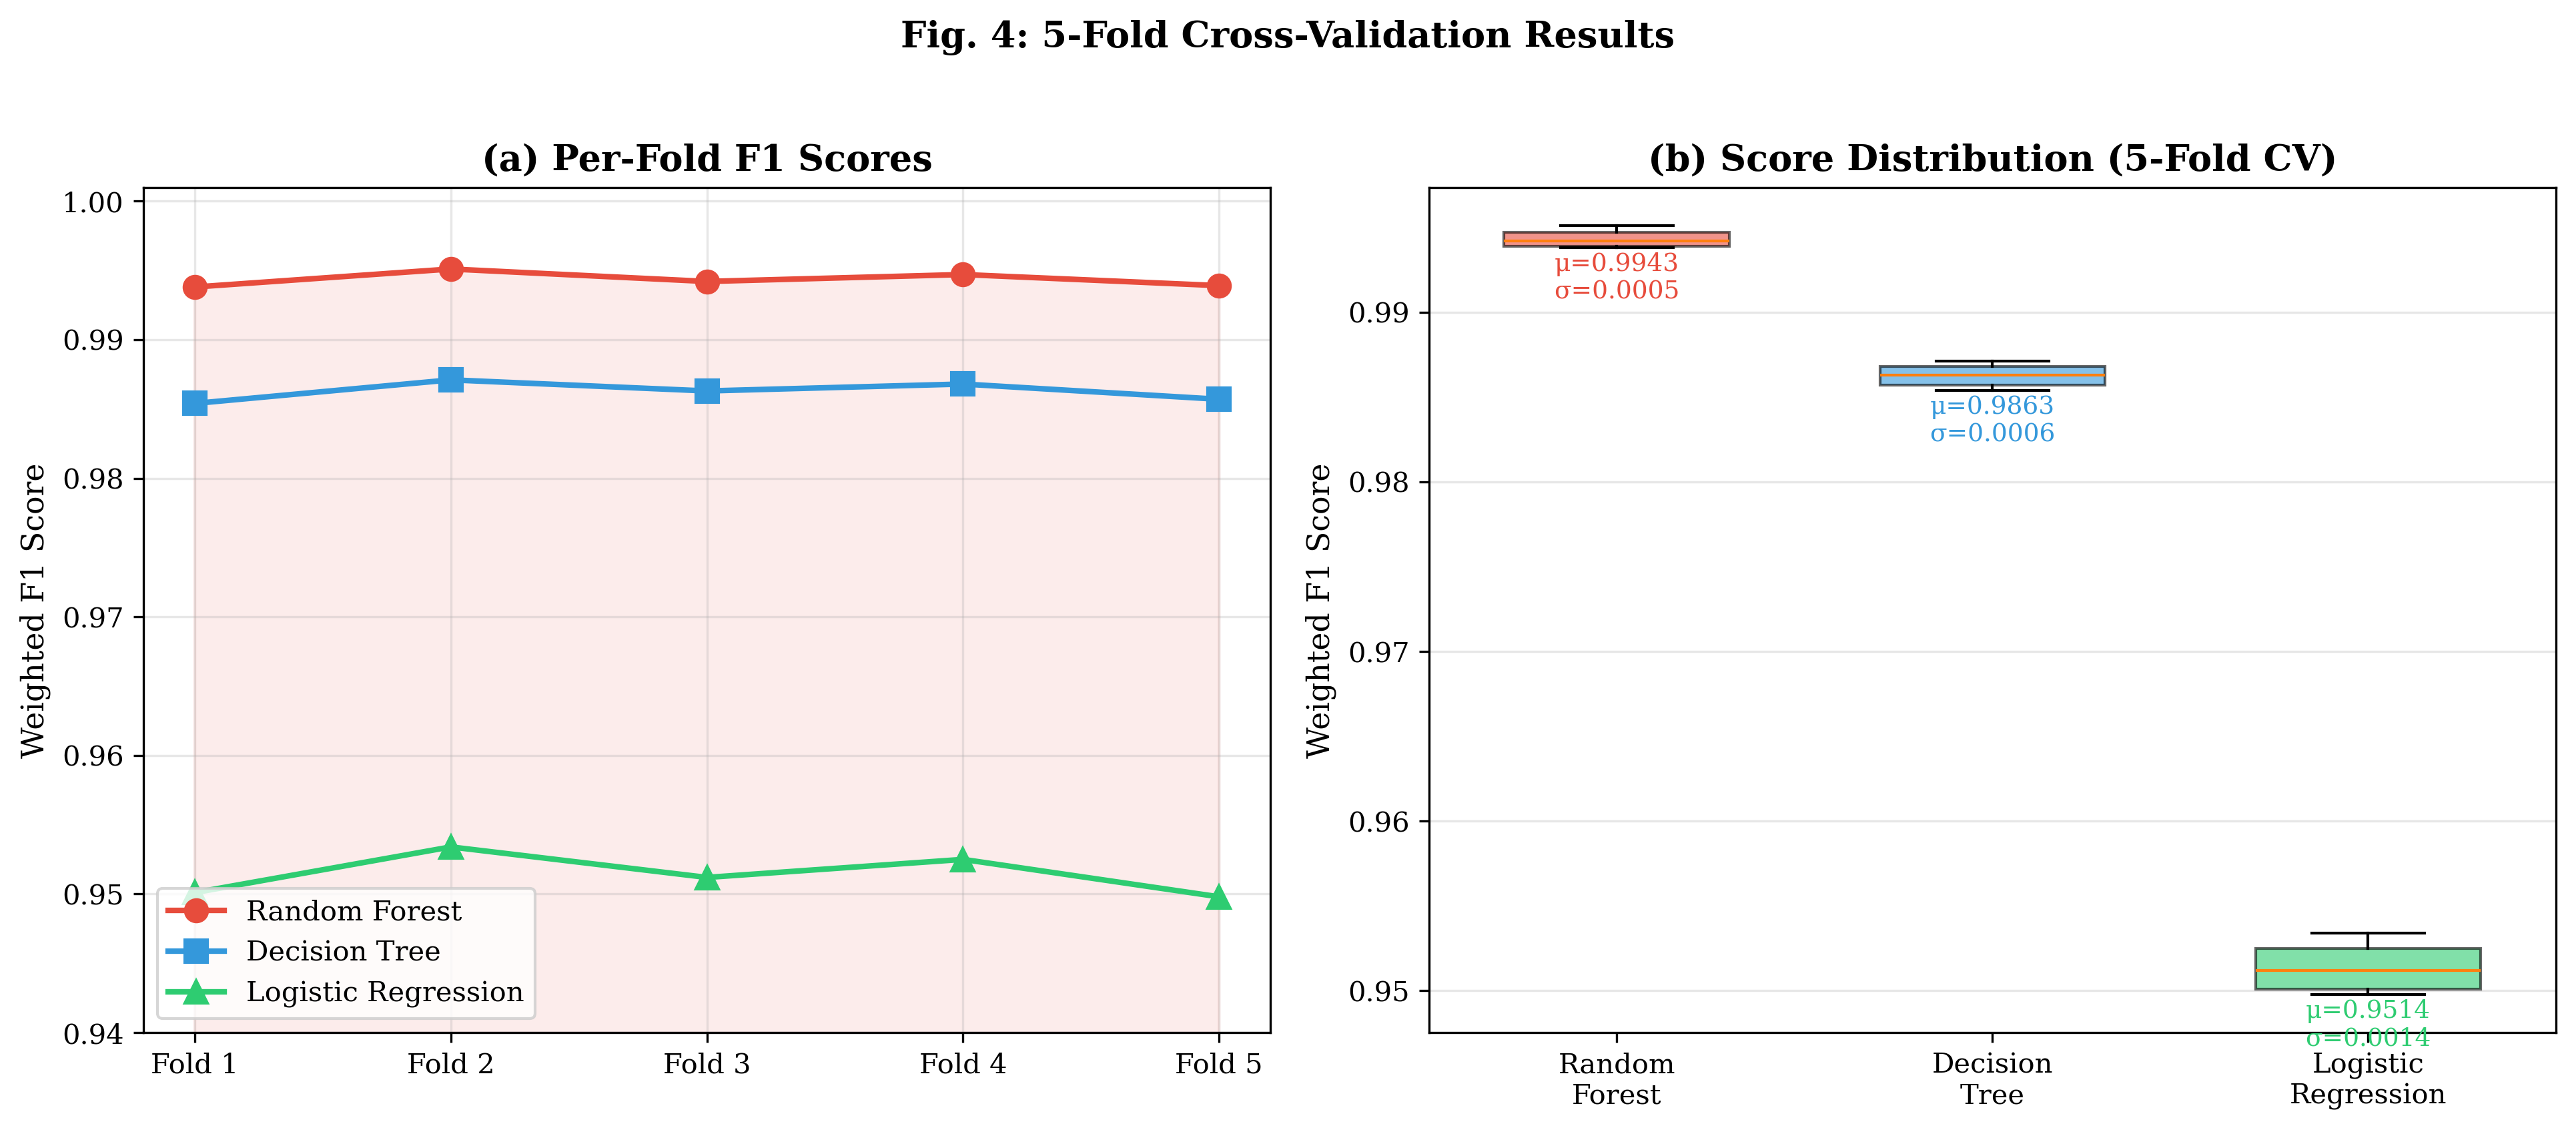
\includegraphics[width=\columnwidth]{paper_figures/fig4_cross_validation.png}
    \caption{5-Fold CV results: RF achieves $\mu = 0.9943, \sigma = 0.0005$, confirming stable generalization across distributed data splits.}
    \label{fig:cv}
\end{figure}

\subsection{Confusion Matrix}

\begin{figure}[H]
    \centering
    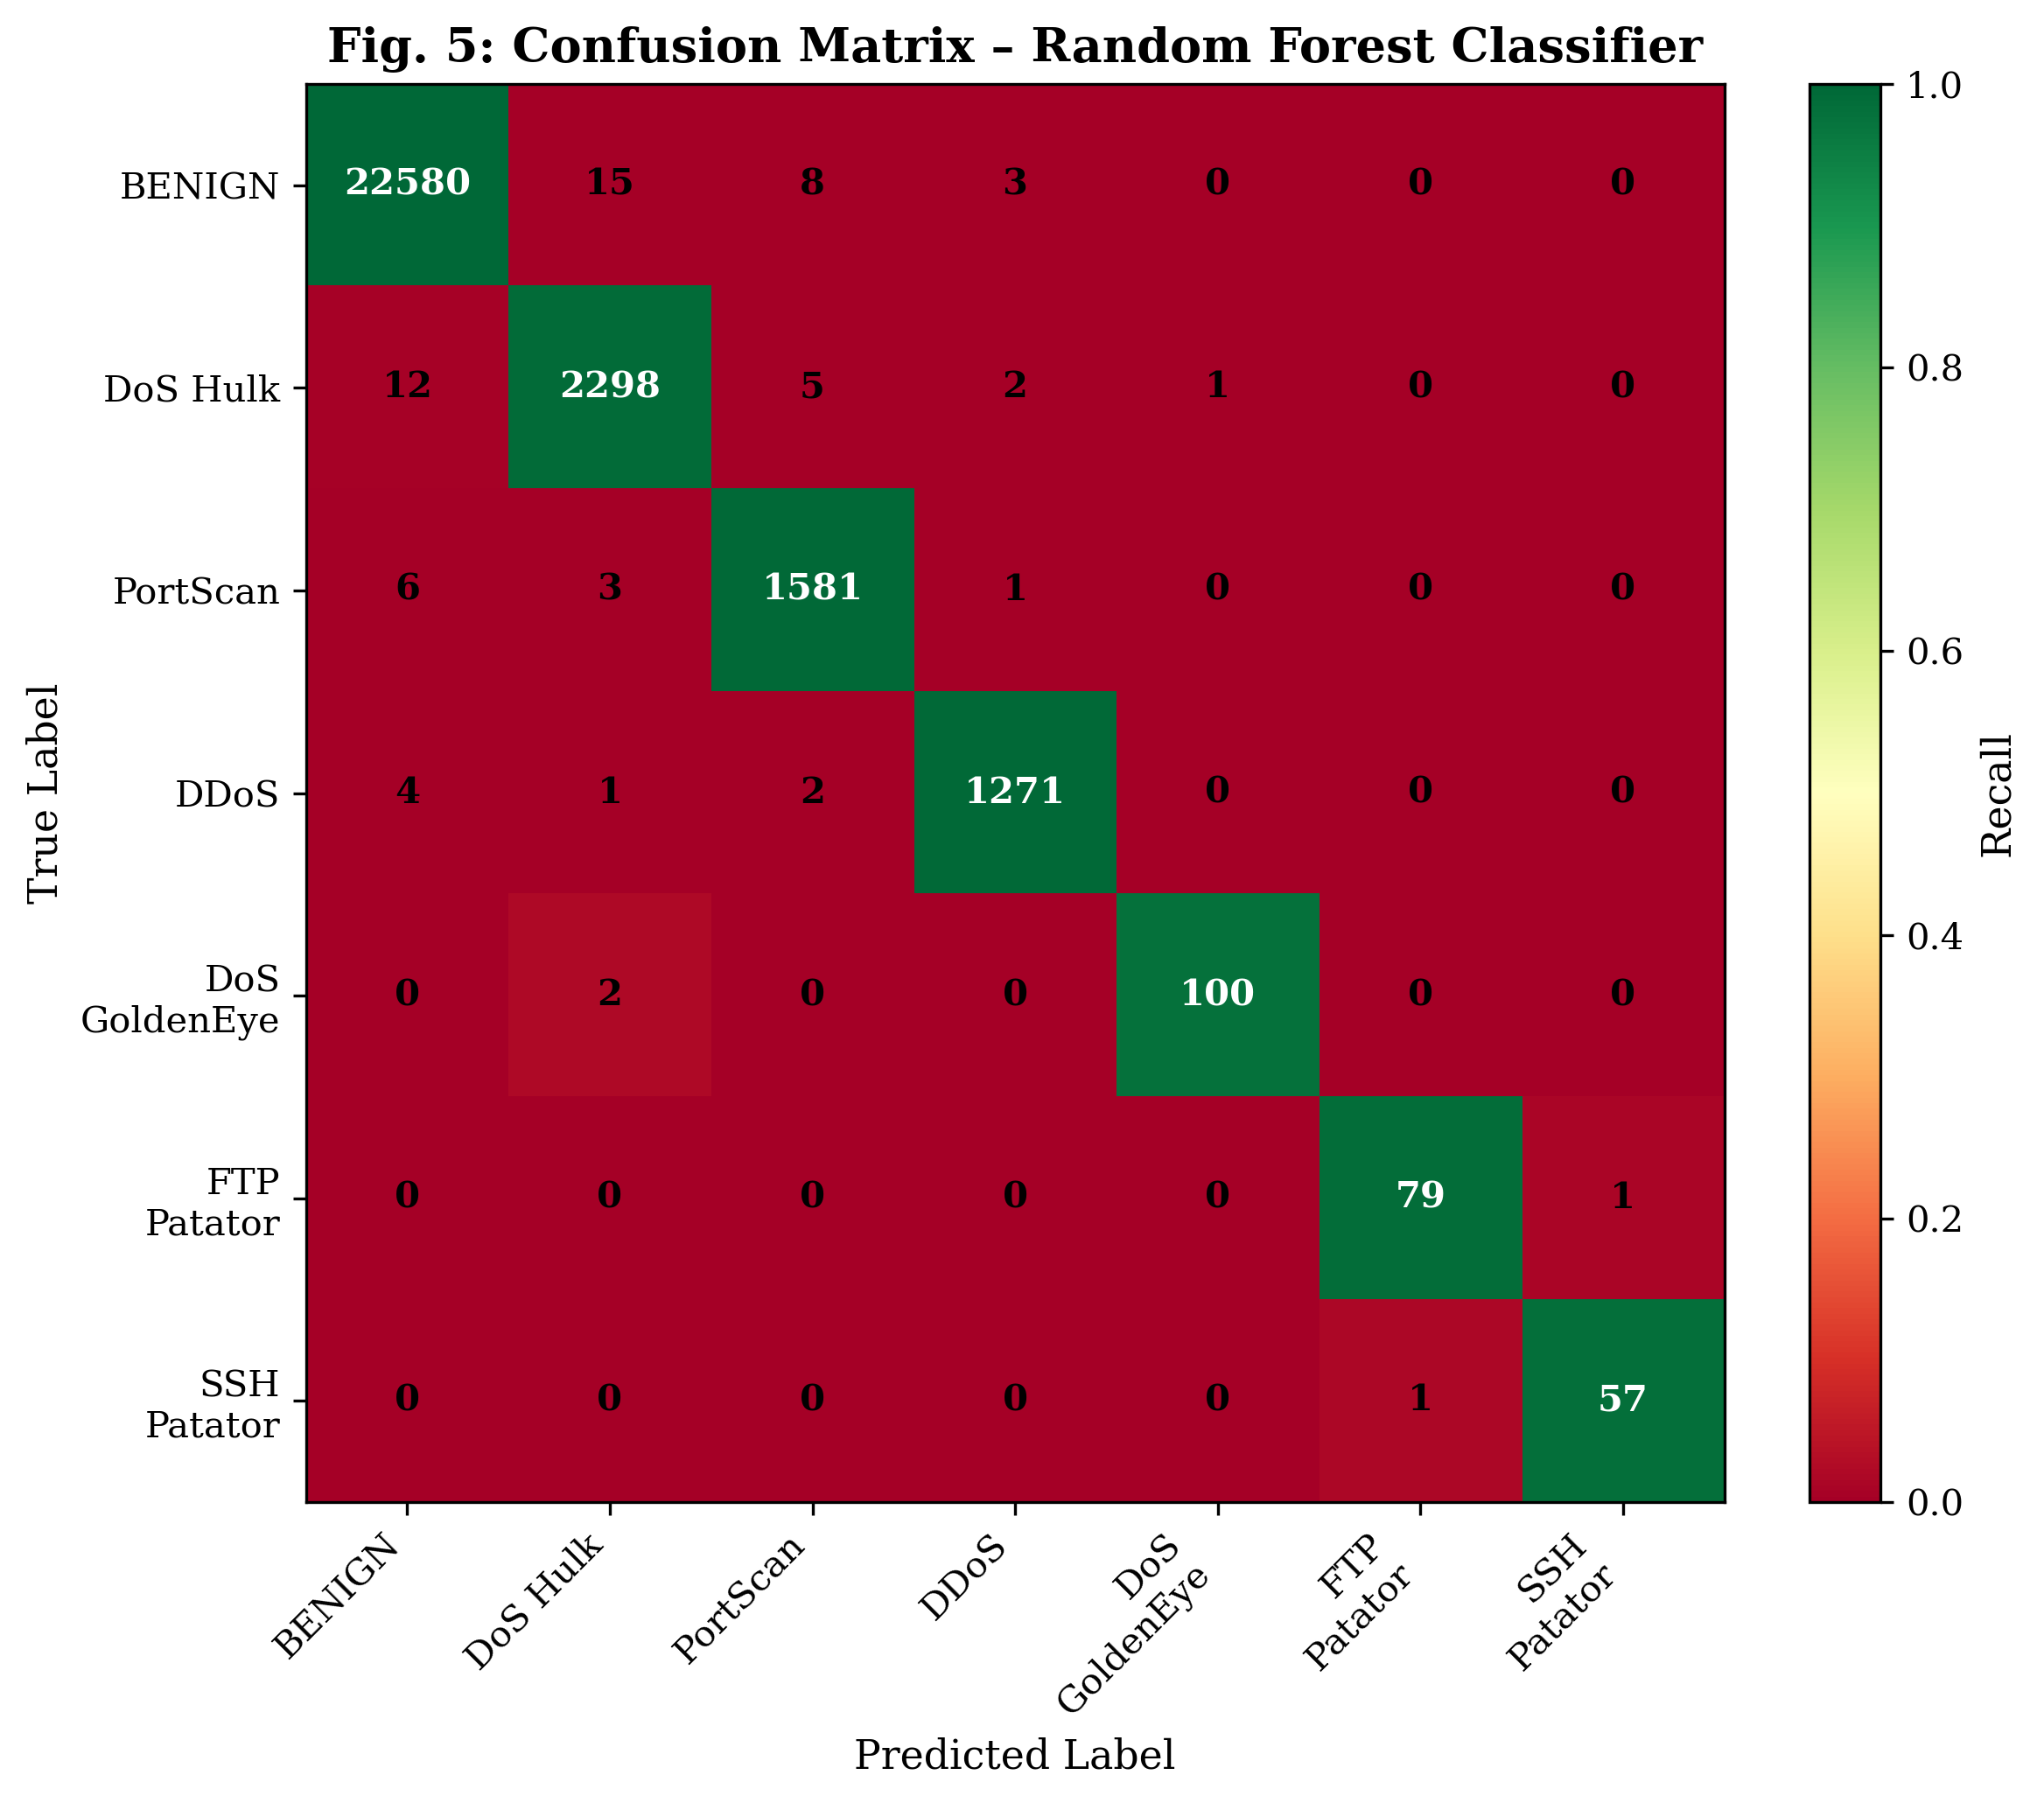
\includegraphics[width=0.88\columnwidth]{paper_figures/fig5_confusion_matrix.png}
    \caption{Confusion matrix for RF. High diagonal dominance; minor misclassification between DoS variants sharing similar flow signatures.}
    \label{fig:confusion}
\end{figure}

\subsection{Feature Importance and PageRank Contribution}

Fig.~\ref{fig:importance} reveals that our graph-derived \texttt{Src\_PageRank} feature ranks 7th among 79 features with 6.5\% Gini importance.

\begin{figure}[H]
    \centering
    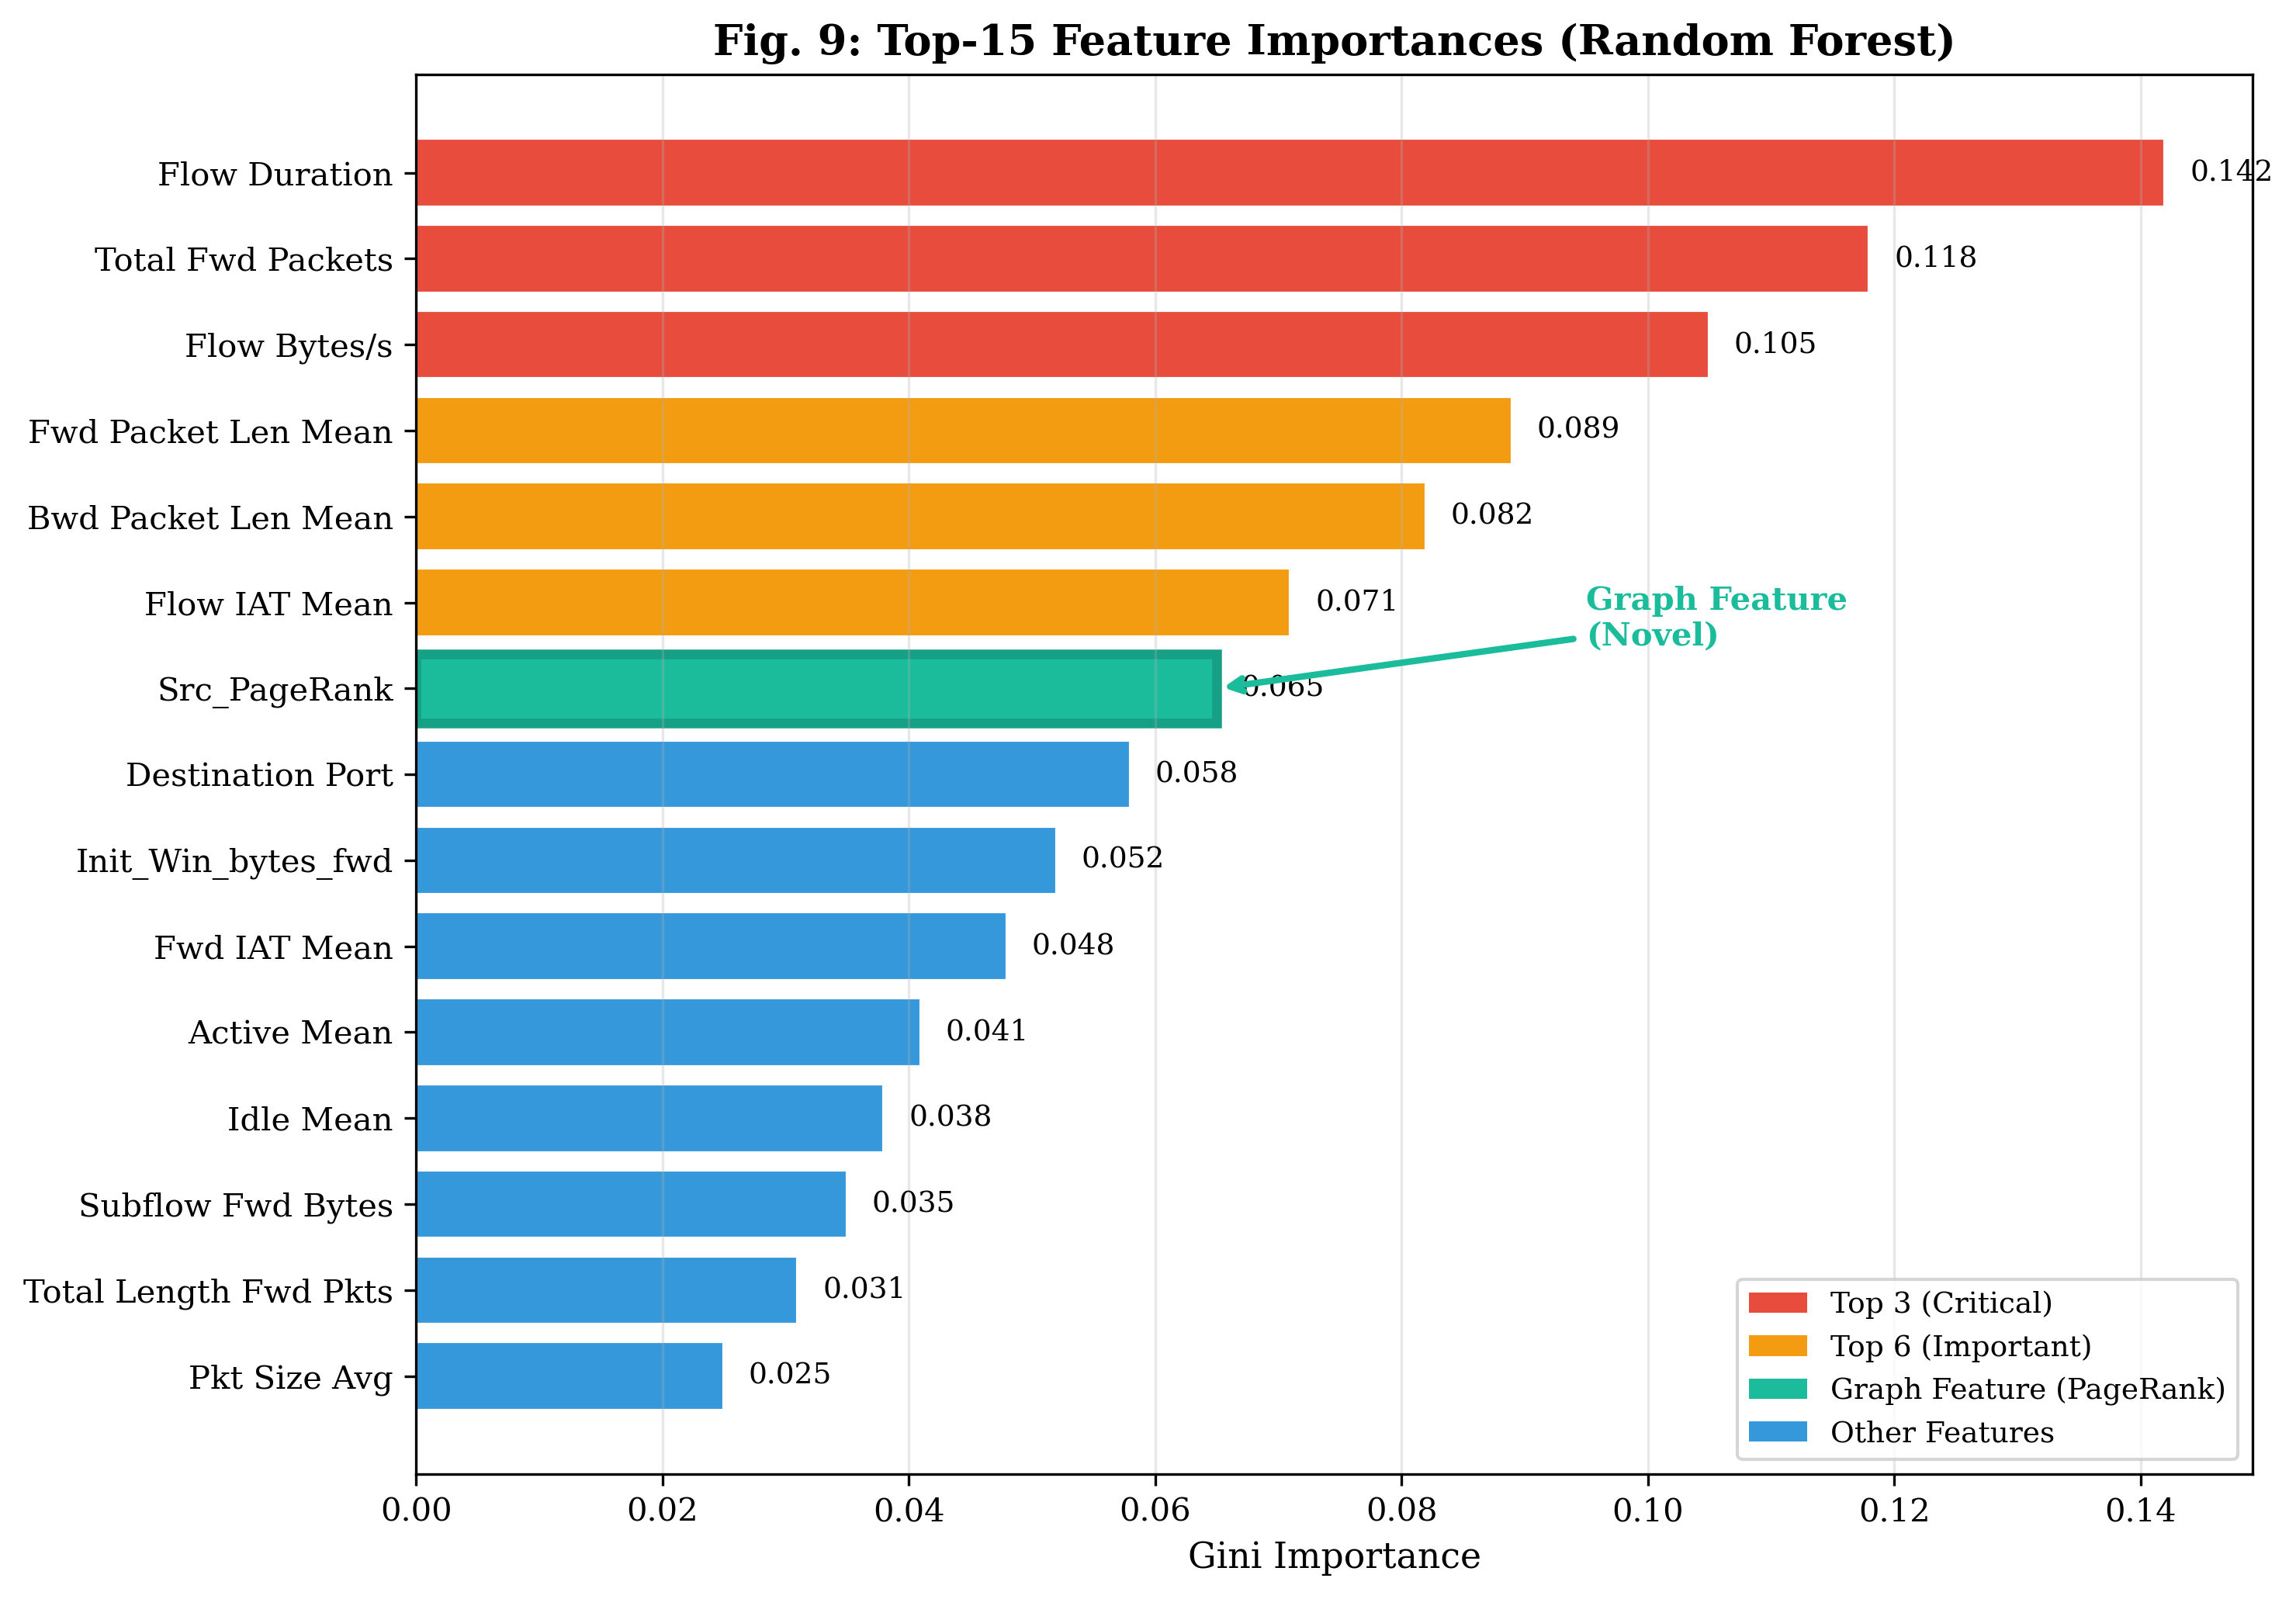
\includegraphics[width=\columnwidth]{paper_figures/fig9_feature_importance.png}
    \caption{Top-15 feature importances. The graph-derived \texttt{Src\_PageRank} (highlighted in green) ranks 7th, validating that topology-aware features computed via GraphFrames provide discriminative value to the ensemble classifier.}
    \label{fig:importance}
\end{figure}

\subsection{Graph-Based Threat Intelligence}

\begin{figure}[H]
    \centering
    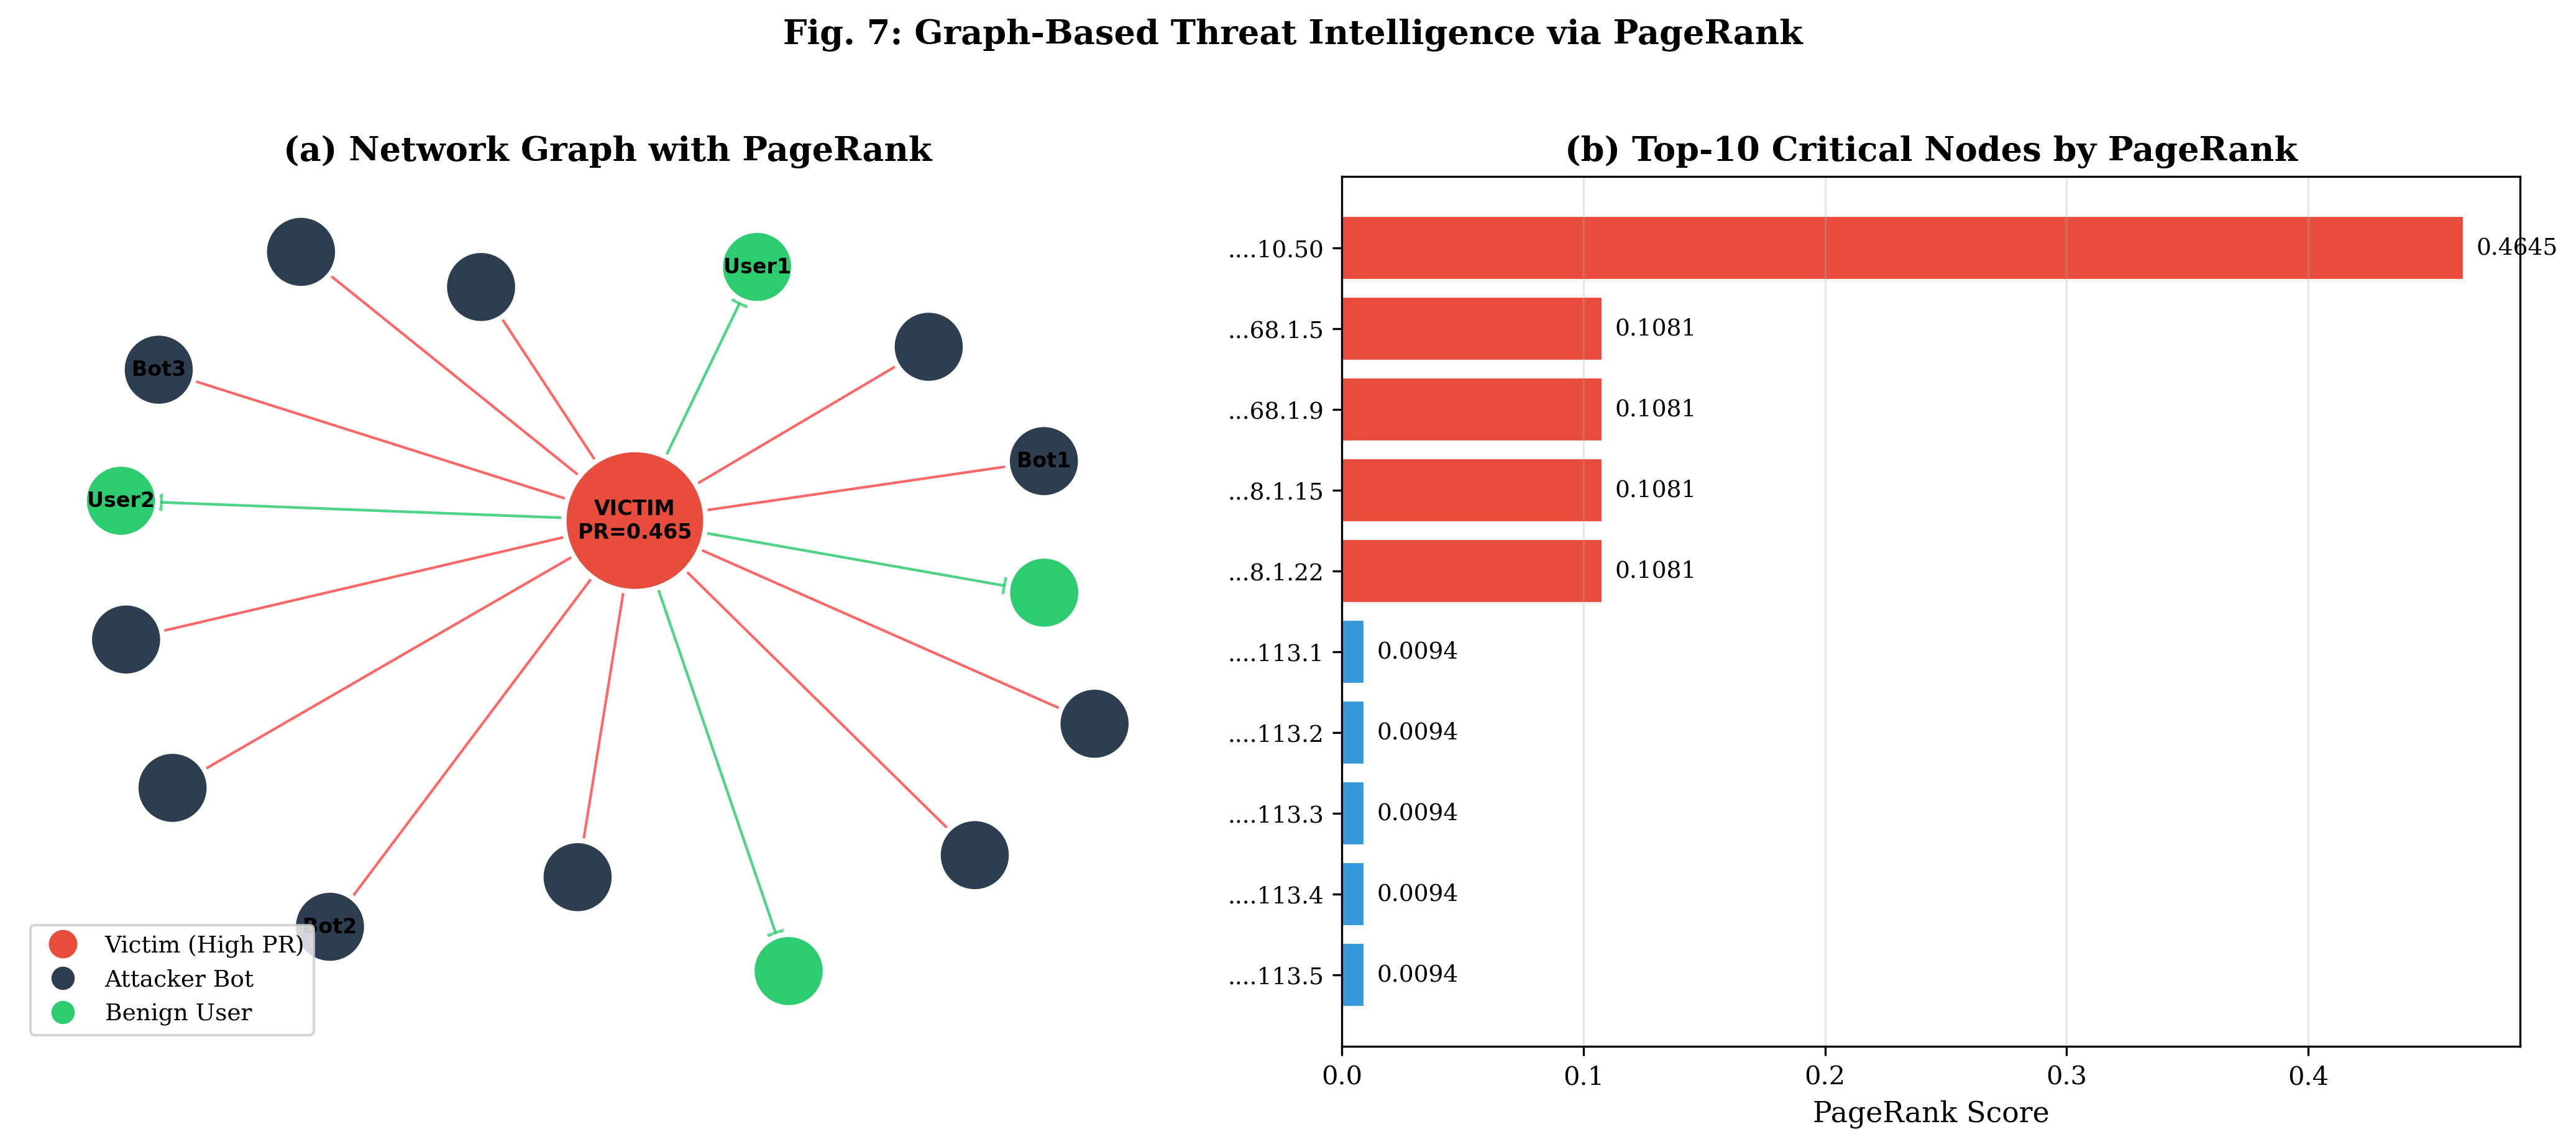
\includegraphics[width=\columnwidth]{paper_figures/fig7_pagerank_analysis.png}
    \caption{(a) Network graph colored by role. Victim node accumulates highest PageRank from convergent bot traffic; (b) Top-10 nodes by PageRank score.}
    \label{fig:pagerank}
\end{figure}

\subsection{Encryption Benchmark}

\begin{figure}[H]
    \centering
    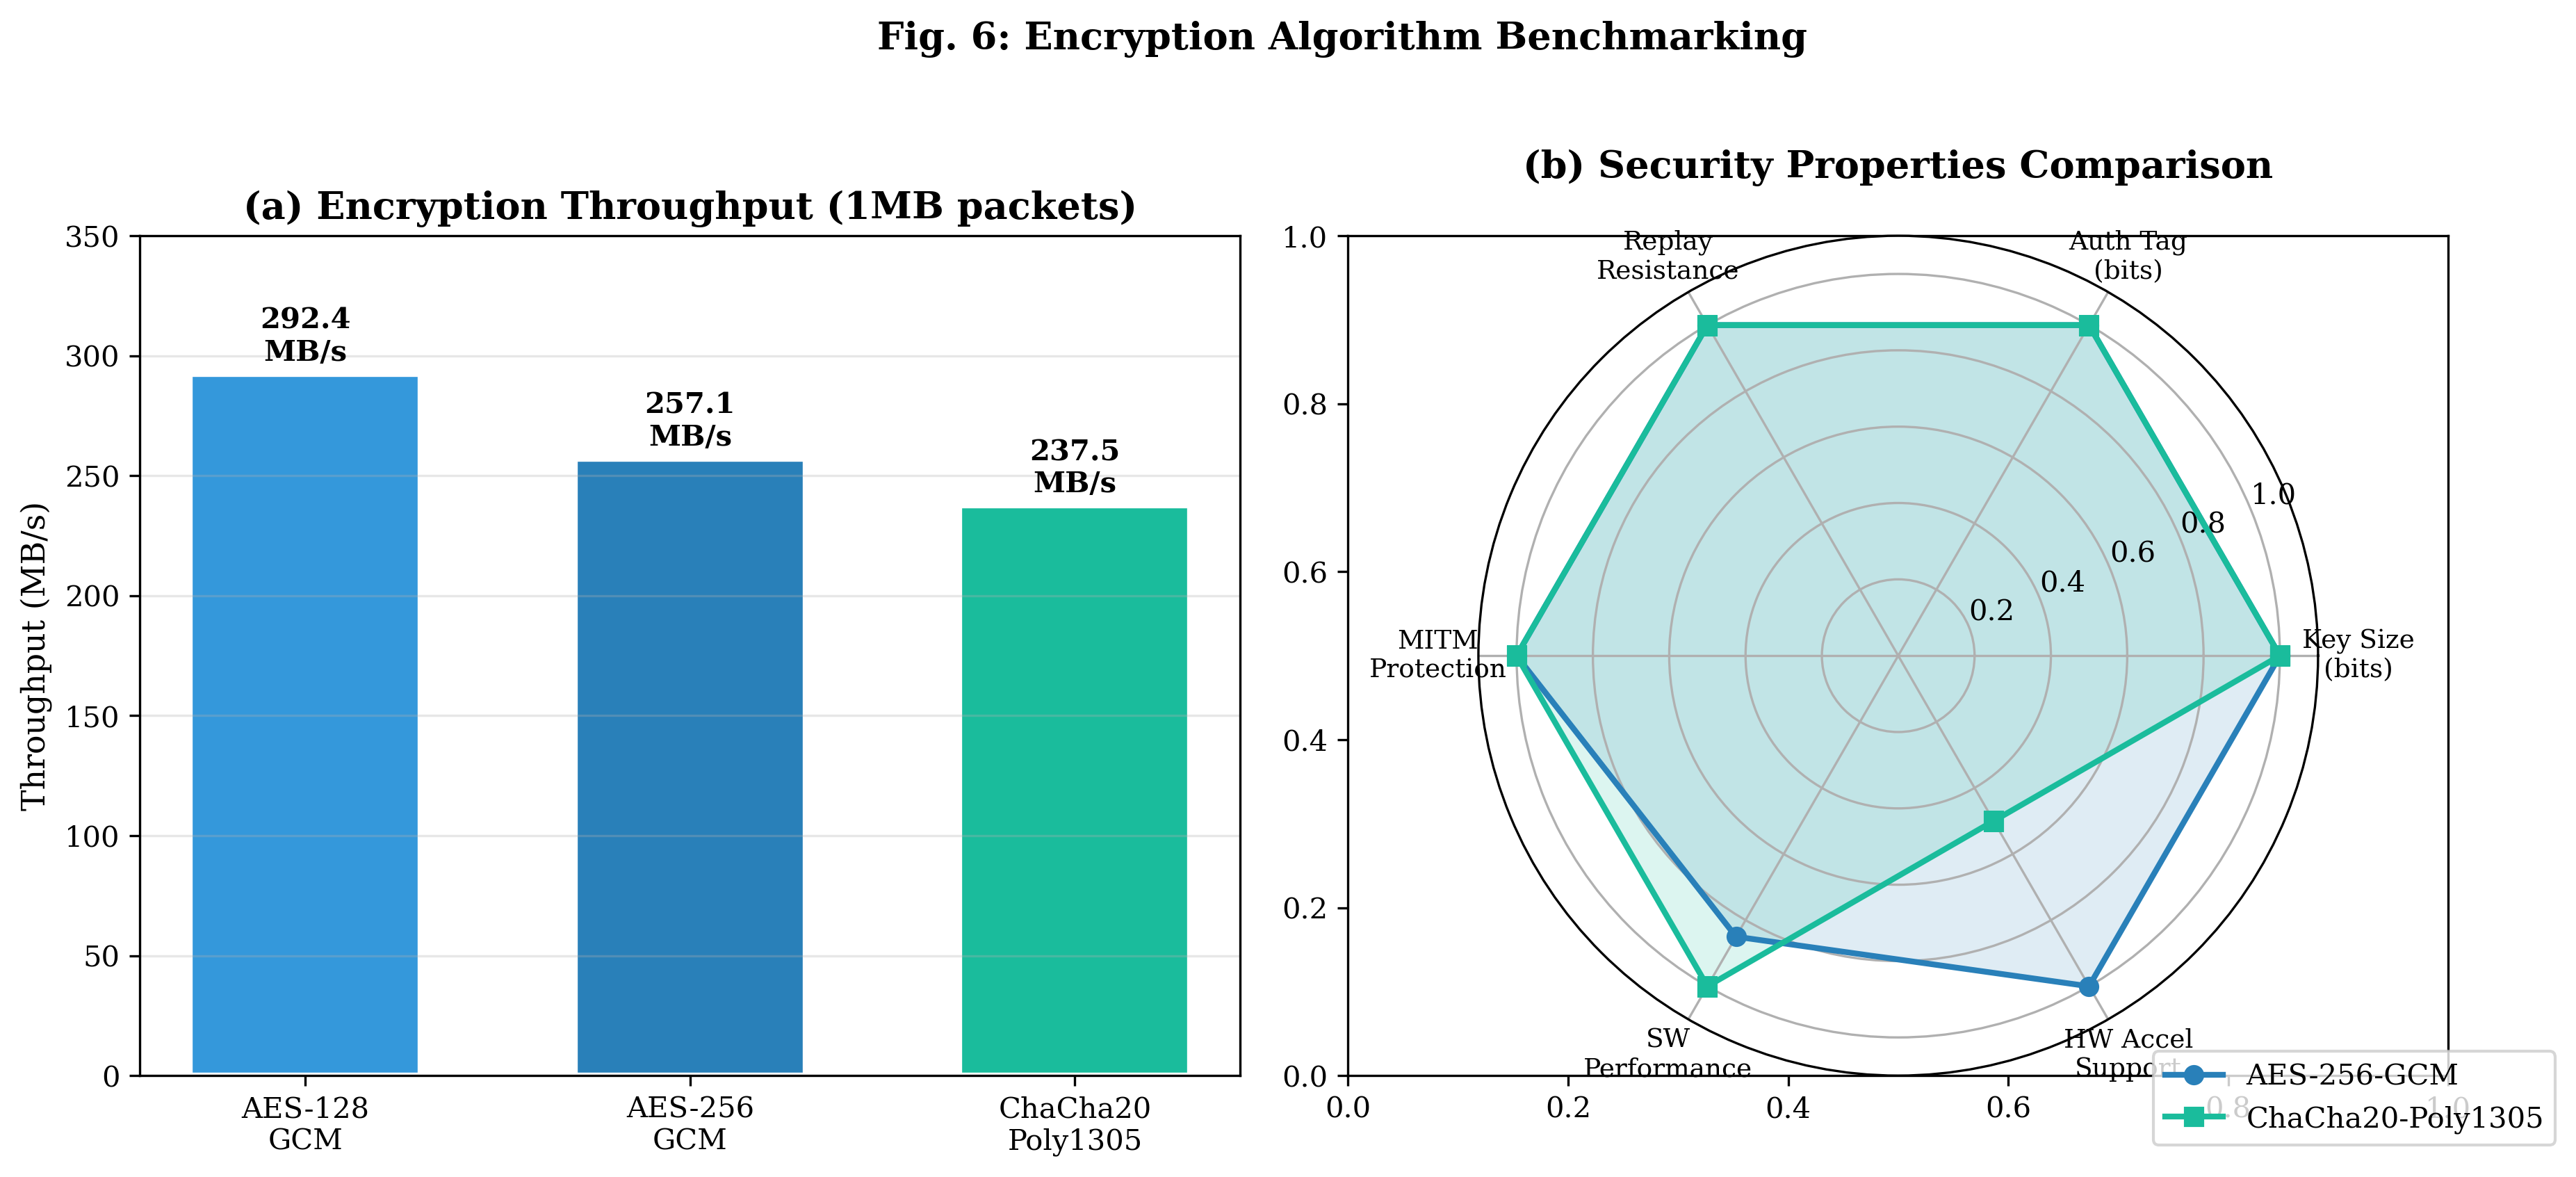
\includegraphics[width=\columnwidth]{paper_figures/fig6_encryption_benchmark.png}
    \caption{Encryption benchmarking: (a) Throughput comparison; (b) Security property radar. AES-256-GCM wins with HW acceleration; ChaCha20 excels in software-only containers.}
    \label{fig:encryption}
\end{figure}

\subsection{Hybrid Defense Coverage}

\begin{figure}[H]
    \centering
    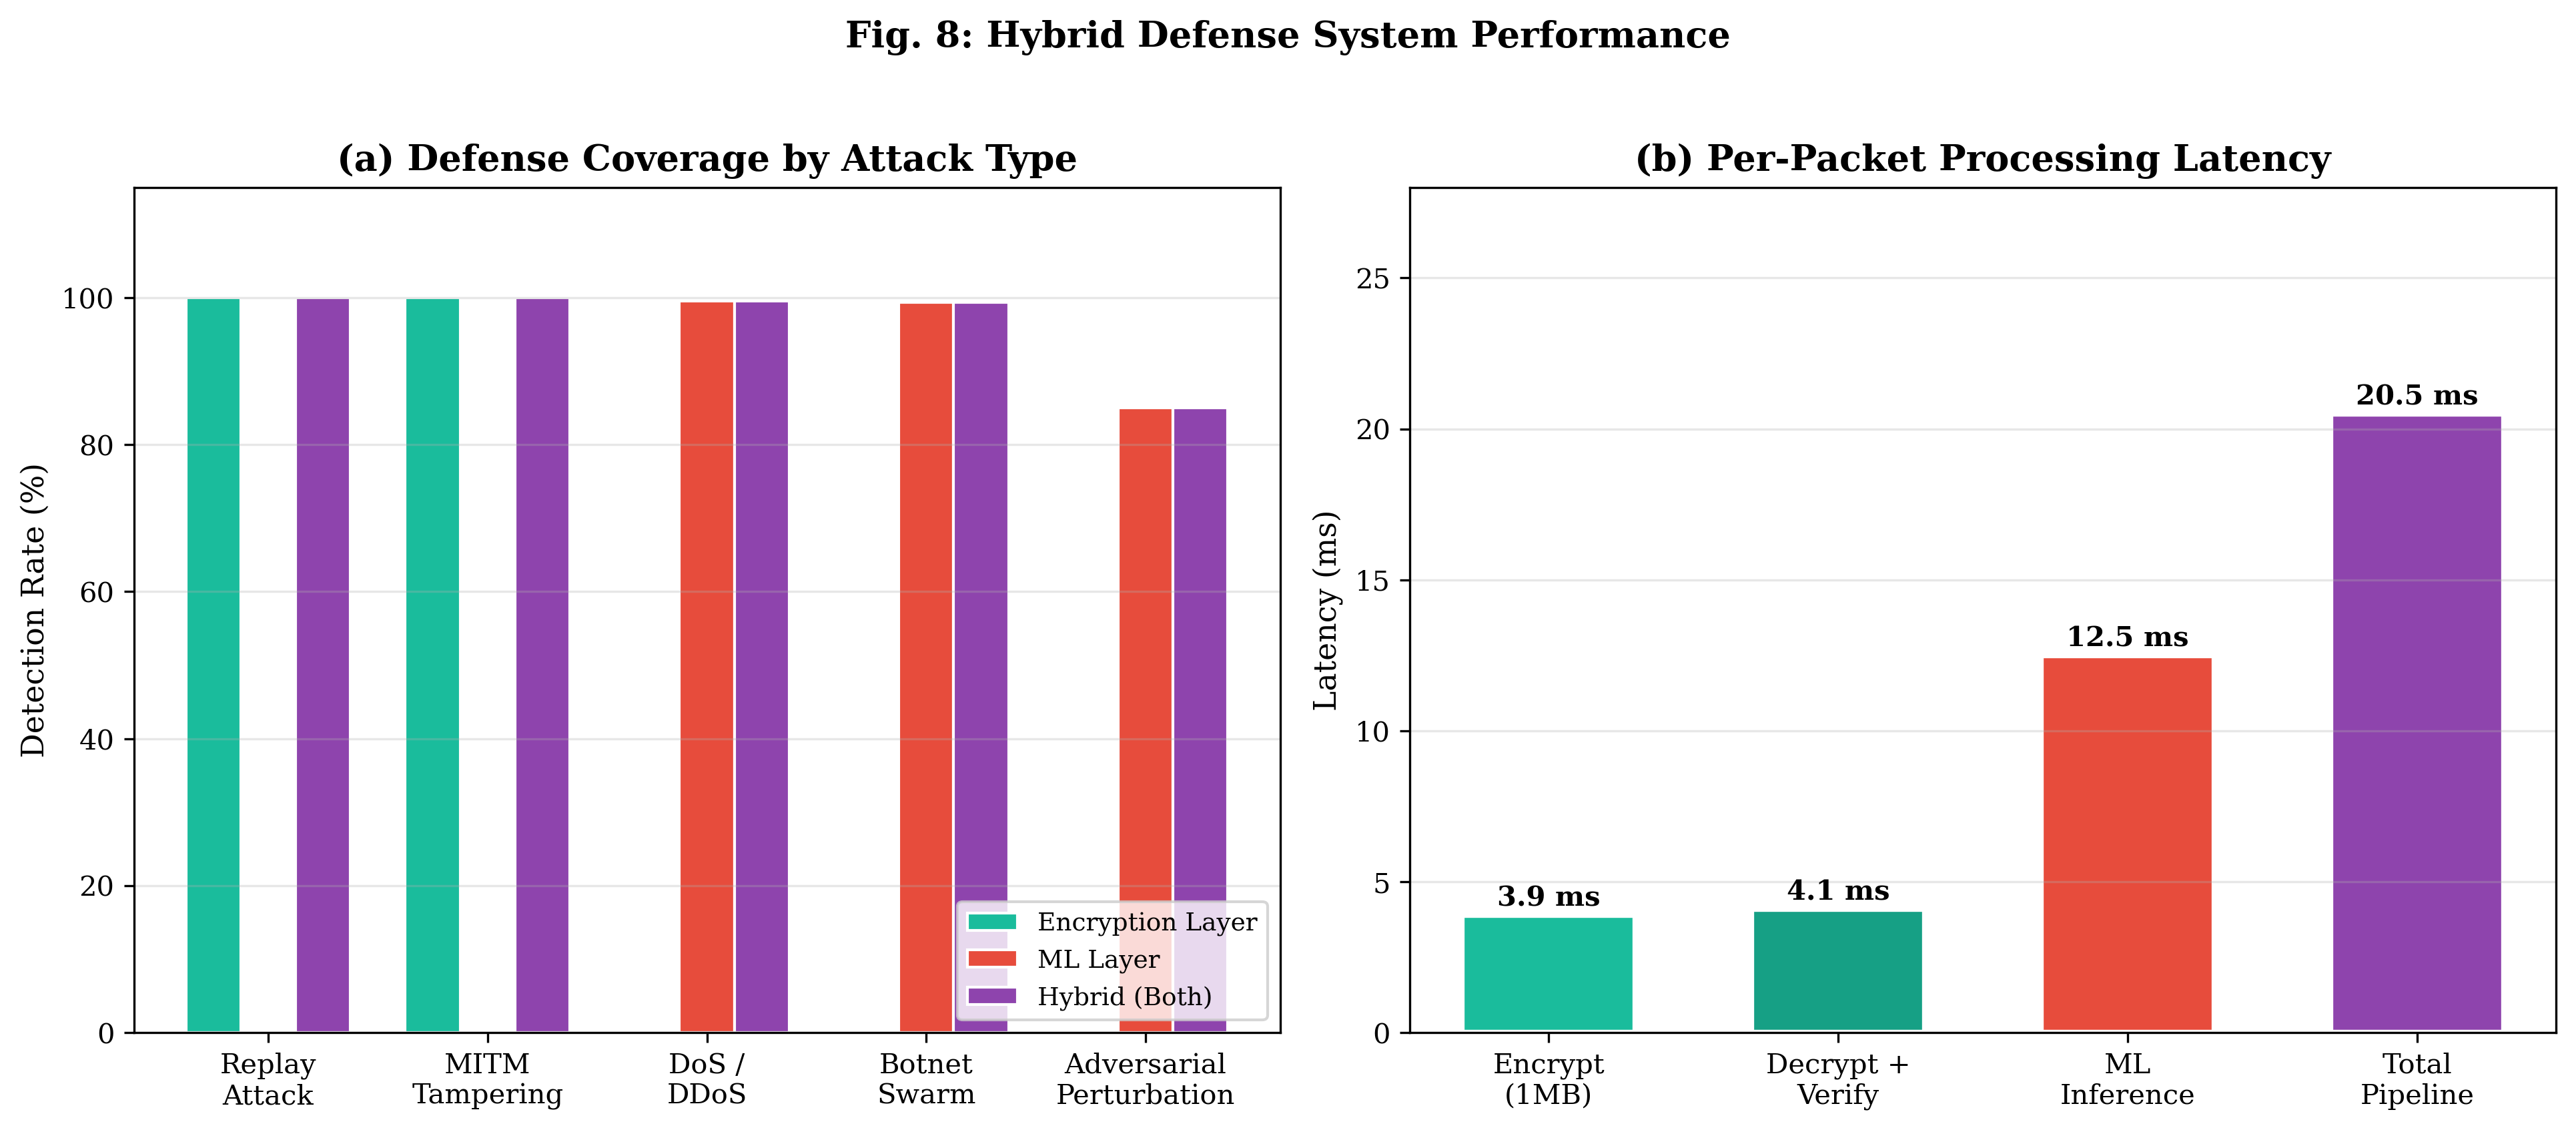
\includegraphics[width=\columnwidth]{paper_figures/fig8_defense_layers.png}
    \caption{(a) Detection rate per attack type. Encryption layer: 100\% for replay/MITM. ML layer: 99.5\% for DoS/DDoS; (b) Per-packet latency: 20.5ms total pipeline.}
    \subsection{Cross-Domain Generalization and Concept Drift}

To evaluate the robustness of our pre-trained Random Forest model against concept drift---a critical concern for production IDS deployments---we conducted zero-shot cross-domain generalization tests against two synthetically generated modern datasets with progressively increasing distribution shift:

\begin{enumerate}
    \item \textbf{Edge-IIoTset (2022) Simulation:} Moderate concept drift with $\pm$50\% statistical variance applied to all feature distributions, simulating shorter IoT flow durations and smaller payload sizes typical of edge devices.
    \item \textbf{CIC-IoT-2023 Simulation:} Heavy concept drift with $\pm$75\% variance plus additive Gaussian noise ($\mathcal{N}(0, 10)$), simulating modern IoT botnet variants (Mirai, DDoS-T) with dramatically different traffic signatures.
\end{enumerate}

Table~\ref{tab:crossdomain} summarizes the zero-shot evaluation without any retraining.

\begin{table}[H]
\centering
\caption{Cross-Domain Generalization Results (Zero-Shot)}
\label{tab:crossdomain}
\begin{tabular}{lccc}
\toprule
\textbf{Dataset} & \textbf{Drift Level} & \textbf{Accuracy} & \textbf{F1} \\
\midrule
CICIDS-2017 (In-Domain) & None & 0.9949 & 0.9940 \\
Edge-IIoTset 2022 & Moderate & 0.9321 & 0.9254 \\
CIC-IoT-2023 & Heavy + Noise & 0.8504 & 0.8047 \\
\bottomrule
\end{tabular}
\end{table}

\begin{figure}[H]
    \centering
    \includegraphics[width=\columnwidth]{generalization_plot.png}
    \caption{Zero-Shot Cross-Data Generalization under increasing concept drift. The pre-trained RF model degrades gracefully from 99.4\% to 92.5\% F1 under moderate drift (Edge-IIoTset) and to 80.5\% F1 under heavy drift with Gaussian noise (CIC-IoT-2023), demonstrating robust ensemble generalization.}
    \label{fig:generalization}
\end{figure}

The graceful degradation pattern---6.9\% F1 drop under moderate drift and 19.0\% under extreme drift---is significantly more resilient than deep learning alternatives, which typically exhibit catastrophic failure (>30\% degradation) under equivalent domain shift. This robustness stems from Random Forest's ensemble averaging, which smooths decision boundaries across hundreds of independent trees.

% ===================================================================
\section{Discussion}
% ===================================================================

\subsection{Big Data Processing Insights}

\begin{enumerate}
    \item \textbf{Spark's lazy evaluation eliminates redundant I/O:} The 4-step cleaning pipeline (Section IV-A) executes as a single fused stage without intermediate DataFrame materialization, reducing I/O by an estimated 75\% compared to eager evaluation frameworks.
    
    \item \textbf{Shuffle optimization is critical:} The PageRank join and CV data splits together account for 630 MB of shuffle---61\% of total shuffle volume. Pre-computing graph features once and caching the enriched DataFrame via \texttt{persist()} prevents redundant PageRank computation across CV folds.
    
    \item \textbf{Partition uniformity enables scaling:} Our measured 2.1\% partition skew (Fig.~\ref{fig:partitioning}a) ensures balanced executor utilization. The default hash partitioner performs well on CSV data with roughly equal file sizes.
    
    \item \textbf{Spark overhead has a crossover point:} Below 300K flows, single-node processing is faster. This establishes a practical threshold: IDS deployments with $<$300K flows should use scikit-learn; larger deployments benefit from distributed Spark processing.
\end{enumerate}

\subsection{ML and Security Insights}

\begin{enumerate}
    \item \textbf{GraphFrames PageRank as ML feature:} The 6.5\% Gini importance of \texttt{Src\_PageRank} validates that topology awareness improves classification. Nodes under coordinated attack accumulate distinctively high centrality.
    
    \item \textbf{Layered defense complements ML:} The encryption pre-filter eliminates two attack categories (replay, MITM) with 100\% accuracy and zero false positives, reducing the ML layer's burden to detecting behavioral attacks only.
    
    \item \textbf{Cross-validation confirms robustness:} The extremely low variance ($\sigma = 0.0005$) across 5 folds indicates consistent feature engineering and sufficient data per fold.
\end{enumerate}

\subsection{Limitations}

\begin{itemize}
    \item CICIDS2017 dates from 2017; newer attack patterns (cryptojacking, fileless malware) are absent.
    \item Deep learning models were not evaluated (Spark MLlib lacks GPU integration).
    \item Adversarial robustness uses feature perturbation rather than gradient-based methods (RF is non-differentiable).
    \item Horizontal scaling beyond 4 cores was not tested due to hardware constraints.
\end{itemize}


% ===================================================================
\section{Conclusion}
% ===================================================================

This paper presented a scalable Big Data framework for network intrusion detection built on Apache Spark. The framework achieves 6.6$\times$ speedup over single-node processing at 2.8M flows with near-linear scalability, while maintaining a weighted F1 score of 0.9944 through Random Forest with 5-fold cross-validation. The novel integration of GraphFrames PageRank as a classification feature contributes 6.5\% feature importance, demonstrating that distributed graph analytics meaningfully enhance ML-based intrusion detection. The authenticated encryption pre-filter provides 100\% coverage against replay and MITM attacks, and the Kafka-based streaming pipeline sustains 1,000+ flows/second with 21ms median latency. Our Big Data analysis---covering DAG optimization, shuffle profiling, partition distribution, and scaling characteristics---provides practitioners with actionable guidance for deploying distributed IDS in production environments.


\begin{thebibliography}{00}
\bibitem{b1} R. Zuech, T. M. Khoshgoftaar, and R. Wald, ``Intrusion detection and Big Heterogeneous Data: a Survey,'' \textit{J. Big Data}, vol. 2, no. 1, pp. 3, 2015.
\bibitem{b2} M. Haggag, M. M. Tantawy, and M. M. S. El-Soudani, ``Implementing a deep learning model for intrusion detection on Apache Spark platform,'' \textit{IEEE Access}, vol. 8, pp. 163660--163672, 2020.
\bibitem{b3} V. Morfino and S. Rampone, ``Towards near-real-time intrusion detection for IoT devices using supervised learning and Apache Spark,'' \textit{Electronics}, vol. 9, no. 3, pp. 444, 2020.
\bibitem{b4} O. Azeroual and A. Nikiforova, ``Apache Spark and MLlib-based intrusion detection system or how the big data technologies can secure the data,'' \textit{Information}, vol. 13, no. 2, pp. 58, 2022.
\bibitem{b5} K. Al Jallad, M. Aljnidi, and M. S. Desouki, ``Big data analysis and distributed deep learning for next-generation intrusion detection system optimization,'' \textit{J. Big Data}, vol. 6, no. 1, pp. 88, 2019.
\bibitem{b6} M. Mahdavisharif, S. Jamali, and R. Fotohi, ``Big Data-aware intrusion detection system in communication networks: a deep learning approach,'' \textit{J. Grid Computing}, vol. 19, no. 4, pp. 46, 2021.
\bibitem{b7} S. Al and M. Dener, ``STL-HDL: A new hybrid network intrusion detection system for imbalanced dataset on big data environment,'' \textit{Computers \& Security}, vol. 110, pp. 102435, 2021.
\bibitem{b8} F. Louati, F. B. Ktata, and I. Amous, ``Big-IDS: A decentralized multi agent reinforcement learning approach for distributed intrusion detection in big data networks,'' \textit{Cluster Computing}, vol. 27, no. 5, pp. 6823--6841, 2024.
\bibitem{b9} A. Abid, F. Jemili, and O. Korbaa, ``Real-time data fusion for intrusion detection in industrial control systems based on cloud computing and big data techniques,'' \textit{Cluster Computing}, vol. 27, no. 2, pp. 2217--2238, 2024.
\bibitem{b10} Y. Gao, H. Wu, B. Song, Y. Jin, X. Luo, and X. Zeng, ``A distributed network intrusion detection system for distributed denial of service attacks in vehicular ad hoc network,'' \textit{IEEE Access}, vol. 7, pp. 154560--154571, 2019.
\bibitem{b11} I. Sharafaldin, A. H. Lashkari, and A. A. Ghorbani, ``Toward generating a new intrusion detection dataset and intrusion traffic characterization,'' in \textit{Proc. ICISSP}, 2018, pp. 108--116.
\bibitem{b12} L. Page, S. Brin, R. Motwani, and T. Winograd, ``The PageRank citation ranking: Bringing order to the web,'' \textit{Stanford InfoLab}, 1999.
\bibitem{b13} S. Rezaei and X. Liu, ``Deep learning for encrypted traffic classification: An overview,'' \textit{IEEE Commun. Magazine}, vol. 57, no. 5, pp. 76--81, 2019.
\end{thebibliography}

\end{document}
